\documentclass{report}


%%%%%%%%%%%%%%%%%%%%%%%%%%%%%%%%%
% PACKAGE IMPORTS
%%%%%%%%%%%%%%%%%%%%%%%%%%%%%%%%%


\usepackage[tmargin=2cm,rmargin=1in,lmargin=1in,margin=0.85in,bmargin=2cm,footskip=.2in]{geometry}
\usepackage{amsmath,amsfonts,amsthm,amssymb,mathtools}
\usepackage[varbb]{newpxmath}
\usepackage{xfrac}
\usepackage[makeroom]{cancel}
\usepackage{mathtools}
\usepackage{bookmark}
\usepackage{enumitem}
\usepackage{hyperref,theoremref}
\hypersetup{
	pdftitle={Assignment},
	colorlinks=true, linkcolor=doc!90,
	bookmarksnumbered=true,
	bookmarksopen=true
}
\usepackage[most,many,breakable]{tcolorbox}
\usepackage{xcolor}
\usepackage{varwidth}
\usepackage{varwidth}
\usepackage{etoolbox}
%\usepackage{authblk}
\usepackage{nameref}
\usepackage{multicol,array}
\usepackage{tikz-cd}
\usepackage[ruled,vlined,linesnumbered]{algorithm2e}
\usepackage{comment} % enables the use of multi-line comments (\ifx \fi) 
\usepackage{import}
\usepackage{xifthen}
\usepackage{pdfpages}
\usepackage{transparent}

\newcommand\mycommfont[1]{\footnotesize\ttfamily\textcolor{blue}{#1}}
\SetCommentSty{mycommfont}
\newcommand{\incfig}[1]{%
    \def\svgwidth{\columnwidth}
    \import{./figures/}{#1.pdf_tex}
}

\usepackage{tikzsymbols}
\renewcommand\qedsymbol{$\Laughey$}


%\usepackage{import}
%\usepackage{xifthen}
%\usepackage{pdfpages}
%\usepackage{transparent}


%%%%%%%%%%%%%%%%%%%%%%%%%%%%%%
% SELF MADE COLORS
%%%%%%%%%%%%%%%%%%%%%%%%%%%%%%



\definecolor{myg}{RGB}{56, 140, 70}
\definecolor{myb}{RGB}{45, 111, 177}
\definecolor{myr}{RGB}{199, 68, 64}
\definecolor{mytheorembg}{HTML}{F2F2F9}
\definecolor{mytheoremfr}{HTML}{00007B}
\definecolor{mylenmabg}{HTML}{FFFAF8}
\definecolor{mylenmafr}{HTML}{983b0f}
\definecolor{mypropbg}{HTML}{f2fbfc}
\definecolor{mypropfr}{HTML}{191971}
\definecolor{myexamplebg}{HTML}{F2FBF8}
\definecolor{myexamplefr}{HTML}{88D6D1}
\definecolor{myexampleti}{HTML}{2A7F7F}
\definecolor{mydefinitbg}{HTML}{E5E5FF}
\definecolor{mydefinitfr}{HTML}{3F3FA3}
\definecolor{notesgreen}{RGB}{0,162,0}
\definecolor{myp}{RGB}{197, 92, 212}
\definecolor{mygr}{HTML}{2C3338}
\definecolor{myred}{RGB}{127,0,0}
\definecolor{myyellow}{RGB}{169,121,69}
\definecolor{myexercisebg}{HTML}{F2FBF8}
\definecolor{myexercisefg}{HTML}{88D6D1}


%%%%%%%%%%%%%%%%%%%%%%%%%%%%
% TCOLORBOX SETUPS
%%%%%%%%%%%%%%%%%%%%%%%%%%%%

\setlength{\parindent}{1cm}
%================================
% THEOREM BOX
%================================

\tcbuselibrary{theorems,skins,hooks}
\newtcbtheorem[number within=section]{Theorem}{Theorem}
{%
	enhanced,
	breakable,
	colback = mytheorembg,
	frame hidden,
	boxrule = 0sp,
	borderline west = {2pt}{0pt}{mytheoremfr},
	sharp corners,
	detach title,
	before upper = \tcbtitle\par\smallskip,
	coltitle = mytheoremfr,
	fonttitle = \bfseries\sffamily,
	description font = \mdseries,
	separator sign none,
	segmentation style={solid, mytheoremfr},
}
{th}

\tcbuselibrary{theorems,skins,hooks}
\newtcbtheorem[number within=chapter]{theorem}{Theorem}
{%
	enhanced,
	breakable,
	colback = mytheorembg,
	frame hidden,
	boxrule = 0sp,
	borderline west = {2pt}{0pt}{mytheoremfr},
	sharp corners,
	detach title,
	before upper = \tcbtitle\par\smallskip,
	coltitle = mytheoremfr,
	fonttitle = \bfseries\sffamily,
	description font = \mdseries,
	separator sign none,
	segmentation style={solid, mytheoremfr},
}
{th}


\tcbuselibrary{theorems,skins,hooks}
\newtcolorbox{Theoremcon}
{%
	enhanced
	,breakable
	,colback = mytheorembg
	,frame hidden
	,boxrule = 0sp
	,borderline west = {2pt}{0pt}{mytheoremfr}
	,sharp corners
	,description font = \mdseries
	,separator sign none
}

%================================
% Corollery
%================================
\tcbuselibrary{theorems,skins,hooks}
\newtcbtheorem[number within=section]{Corollary}{Corollary}
{%
	enhanced
	,breakable
	,colback = myp!10
	,frame hidden
	,boxrule = 0sp
	,borderline west = {2pt}{0pt}{myp!85!black}
	,sharp corners
	,detach title
	,before upper = \tcbtitle\par\smallskip
	,coltitle = myp!85!black
	,fonttitle = \bfseries\sffamily
	,description font = \mdseries
	,separator sign none
	,segmentation style={solid, myp!85!black}
}
{th}
\tcbuselibrary{theorems,skins,hooks}
\newtcbtheorem[number within=chapter]{corollary}{Corollary}
{%
	enhanced
	,breakable
	,colback = myp!10
	,frame hidden
	,boxrule = 0sp
	,borderline west = {2pt}{0pt}{myp!85!black}
	,sharp corners
	,detach title
	,before upper = \tcbtitle\par\smallskip
	,coltitle = myp!85!black
	,fonttitle = \bfseries\sffamily
	,description font = \mdseries
	,separator sign none
	,segmentation style={solid, myp!85!black}
}
{th}


%================================
% LENMA
%================================

\tcbuselibrary{theorems,skins,hooks}
\newtcbtheorem[number within=section]{Lenma}{Lenma}
{%
	enhanced,
	breakable,
	colback = mylenmabg,
	frame hidden,
	boxrule = 0sp,
	borderline west = {2pt}{0pt}{mylenmafr},
	sharp corners,
	detach title,
	before upper = \tcbtitle\par\smallskip,
	coltitle = mylenmafr,
	fonttitle = \bfseries\sffamily,
	description font = \mdseries,
	separator sign none,
	segmentation style={solid, mylenmafr},
}
{th}

\tcbuselibrary{theorems,skins,hooks}
\newtcbtheorem[number within=chapter]{lenma}{Lenma}
{%
	enhanced,
	breakable,
	colback = mylenmabg,
	frame hidden,
	boxrule = 0sp,
	borderline west = {2pt}{0pt}{mylenmafr},
	sharp corners,
	detach title,
	before upper = \tcbtitle\par\smallskip,
	coltitle = mylenmafr,
	fonttitle = \bfseries\sffamily,
	description font = \mdseries,
	separator sign none,
	segmentation style={solid, mylenmafr},
}
{th}


%================================
% PROPOSITION
%================================

\tcbuselibrary{theorems,skins,hooks}
\newtcbtheorem[number within=section]{Prop}{Proposition}
{%
	enhanced,
	breakable,
	colback = mypropbg,
	frame hidden,
	boxrule = 0sp,
	borderline west = {2pt}{0pt}{mypropfr},
	sharp corners,
	detach title,
	before upper = \tcbtitle\par\smallskip,
	coltitle = mypropfr,
	fonttitle = \bfseries\sffamily,
	description font = \mdseries,
	separator sign none,
	segmentation style={solid, mypropfr},
}
{th}

\tcbuselibrary{theorems,skins,hooks}
\newtcbtheorem[number within=chapter]{prop}{Proposition}
{%
	enhanced,
	breakable,
	colback = mypropbg,
	frame hidden,
	boxrule = 0sp,
	borderline west = {2pt}{0pt}{mypropfr},
	sharp corners,
	detach title,
	before upper = \tcbtitle\par\smallskip,
	coltitle = mypropfr,
	fonttitle = \bfseries\sffamily,
	description font = \mdseries,
	separator sign none,
	segmentation style={solid, mypropfr},
}
{th}


%================================
% CLAIM
%================================

\tcbuselibrary{theorems,skins,hooks}
\newtcbtheorem[number within=section]{claim}{Claim}
{%
	enhanced
	,breakable
	,colback = myg!10
	,frame hidden
	,boxrule = 0sp
	,borderline west = {2pt}{0pt}{myg}
	,sharp corners
	,detach title
	,before upper = \tcbtitle\par\smallskip
	,coltitle = myg!85!black
	,fonttitle = \bfseries\sffamily
	,description font = \mdseries
	,separator sign none
	,segmentation style={solid, myg!85!black}
}
{th}



%================================
% Exercise
%================================

\tcbuselibrary{theorems,skins,hooks}
\newtcbtheorem[number within=section]{Exercise}{Exercise}
{%
	enhanced,
	breakable,
	colback = myexercisebg,
	frame hidden,
	boxrule = 0sp,
	borderline west = {2pt}{0pt}{myexercisefg},
	sharp corners,
	detach title,
	before upper = \tcbtitle\par\smallskip,
	coltitle = myexercisefg,
	fonttitle = \bfseries\sffamily,
	description font = \mdseries,
	separator sign none,
	segmentation style={solid, myexercisefg},
}
{th}

\tcbuselibrary{theorems,skins,hooks}
\newtcbtheorem[number within=chapter]{exercise}{Exercise}
{%
	enhanced,
	breakable,
	colback = myexercisebg,
	frame hidden,
	boxrule = 0sp,
	borderline west = {2pt}{0pt}{myexercisefg},
	sharp corners,
	detach title,
	before upper = \tcbtitle\par\smallskip,
	coltitle = myexercisefg,
	fonttitle = \bfseries\sffamily,
	description font = \mdseries,
	separator sign none,
	segmentation style={solid, myexercisefg},
}
{th}

%================================
% EXAMPLE BOX
%================================

\newtcbtheorem[number within=section]{Example}{Example}
{%
	colback = myexamplebg
	,breakable
	,colframe = myexamplefr
	,coltitle = myexampleti
	,boxrule = 1pt
	,sharp corners
	,detach title
	,before upper=\tcbtitle\par\smallskip
	,fonttitle = \bfseries
	,description font = \mdseries
	,separator sign none
	,description delimiters parenthesis
}
{ex}

\newtcbtheorem[number within=chapter]{example}{Example}
{%
	colback = myexamplebg
	,breakable
	,colframe = myexamplefr
	,coltitle = myexampleti
	,boxrule = 1pt
	,sharp corners
	,detach title
	,before upper=\tcbtitle\par\smallskip
	,fonttitle = \bfseries
	,description font = \mdseries
	,separator sign none
	,description delimiters parenthesis
}
{ex}

%================================
% DEFINITION BOX
%================================

\newtcbtheorem[number within=section]{Definition}{Definition}{enhanced,
	before skip=2mm,after skip=2mm, colback=red!5,colframe=red!80!black,boxrule=0.5mm,
	attach boxed title to top left={xshift=1cm,yshift*=1mm-\tcboxedtitleheight}, varwidth boxed title*=-3cm,
	boxed title style={frame code={
					\path[fill=tcbcolback]
					([yshift=-1mm,xshift=-1mm]frame.north west)
					arc[start angle=0,end angle=180,radius=1mm]
					([yshift=-1mm,xshift=1mm]frame.north east)
					arc[start angle=180,end angle=0,radius=1mm];
					\path[left color=tcbcolback!60!black,right color=tcbcolback!60!black,
						middle color=tcbcolback!80!black]
					([xshift=-2mm]frame.north west) -- ([xshift=2mm]frame.north east)
					[rounded corners=1mm]-- ([xshift=1mm,yshift=-1mm]frame.north east)
					-- (frame.south east) -- (frame.south west)
					-- ([xshift=-1mm,yshift=-1mm]frame.north west)
					[sharp corners]-- cycle;
				},interior engine=empty,
		},
	fonttitle=\bfseries,
	title={#2},#1}{def}
\newtcbtheorem[number within=chapter]{definition}{Definition}{enhanced,
	before skip=2mm,after skip=2mm, colback=red!5,colframe=red!80!black,boxrule=0.5mm,
	attach boxed title to top left={xshift=1cm,yshift*=1mm-\tcboxedtitleheight}, varwidth boxed title*=-3cm,
	boxed title style={frame code={
					\path[fill=tcbcolback]
					([yshift=-1mm,xshift=-1mm]frame.north west)
					arc[start angle=0,end angle=180,radius=1mm]
					([yshift=-1mm,xshift=1mm]frame.north east)
					arc[start angle=180,end angle=0,radius=1mm];
					\path[left color=tcbcolback!60!black,right color=tcbcolback!60!black,
						middle color=tcbcolback!80!black]
					([xshift=-2mm]frame.north west) -- ([xshift=2mm]frame.north east)
					[rounded corners=1mm]-- ([xshift=1mm,yshift=-1mm]frame.north east)
					-- (frame.south east) -- (frame.south west)
					-- ([xshift=-1mm,yshift=-1mm]frame.north west)
					[sharp corners]-- cycle;
				},interior engine=empty,
		},
	fonttitle=\bfseries,
	title={#2},#1}{def}



%================================
% Solution BOX
%================================

\makeatletter
\newtcbtheorem{question}{Question}{enhanced,
	breakable,
	colback=white,
	colframe=myb!80!black,
	attach boxed title to top left={yshift*=-\tcboxedtitleheight},
	fonttitle=\bfseries,
	title={#2},
	boxed title size=title,
	boxed title style={%
			sharp corners,
			rounded corners=northwest,
			colback=tcbcolframe,
			boxrule=0pt,
		},
	underlay boxed title={%
			\path[fill=tcbcolframe] (title.south west)--(title.south east)
			to[out=0, in=180] ([xshift=5mm]title.east)--
			(title.center-|frame.east)
			[rounded corners=\kvtcb@arc] |-
			(frame.north) -| cycle;
		},
	#1
}{def}
\makeatother

%================================
% SOLUTION BOX
%================================

\makeatletter
\newtcolorbox{solution}{enhanced,
	breakable,
	colback=white,
	colframe=myg!80!black,
	attach boxed title to top left={yshift*=-\tcboxedtitleheight},
	title=Solution,
	boxed title size=title,
	boxed title style={%
			sharp corners,
			rounded corners=northwest,
			colback=tcbcolframe,
			boxrule=0pt,
		},
	underlay boxed title={%
			\path[fill=tcbcolframe] (title.south west)--(title.south east)
			to[out=0, in=180] ([xshift=5mm]title.east)--
			(title.center-|frame.east)
			[rounded corners=\kvtcb@arc] |-
			(frame.north) -| cycle;
		},
}
\makeatother

%================================
% Question BOX
%================================

\makeatletter
\newtcbtheorem{qstion}{Question}{enhanced,
	breakable,
	colback=white,
	colframe=mygr,
	attach boxed title to top left={yshift*=-\tcboxedtitleheight},
	fonttitle=\bfseries,
	title={#2},
	boxed title size=title,
	boxed title style={%
			sharp corners,
			rounded corners=northwest,
			colback=tcbcolframe,
			boxrule=0pt,
		},
	underlay boxed title={%
			\path[fill=tcbcolframe] (title.south west)--(title.south east)
			to[out=0, in=180] ([xshift=5mm]title.east)--
			(title.center-|frame.east)
			[rounded corners=\kvtcb@arc] |-
			(frame.north) -| cycle;
		},
	#1
}{def}
\makeatother

\newtcbtheorem[number within=chapter]{wconc}{Wrong Concept}{
	breakable,
	enhanced,
	colback=white,
	colframe=myr,
	arc=0pt,
	outer arc=0pt,
	fonttitle=\bfseries\sffamily\large,
	colbacktitle=myr,
	attach boxed title to top left={},
	boxed title style={
			enhanced,
			skin=enhancedfirst jigsaw,
			arc=3pt,
			bottom=0pt,
			interior style={fill=myr}
		},
	#1
}{def}



%================================
% NOTE BOX
%================================

\usetikzlibrary{arrows,calc,shadows.blur}
\tcbuselibrary{skins}
\newtcolorbox{note}[1][]{%
	enhanced jigsaw,
	colback=gray!20!white,%
	colframe=gray!80!black,
	size=small,
	boxrule=1pt,
	title=\textbf{Note:-},
	halign title=flush center,
	coltitle=black,
	breakable,
	drop shadow=black!50!white,
	attach boxed title to top left={xshift=1cm,yshift=-\tcboxedtitleheight/2,yshifttext=-\tcboxedtitleheight/2},
	minipage boxed title=1.5cm,
	boxed title style={%
			colback=white,
			size=fbox,
			boxrule=1pt,
			boxsep=2pt,
			underlay={%
					\coordinate (dotA) at ($(interior.west) + (-0.5pt,0)$);
					\coordinate (dotB) at ($(interior.east) + (0.5pt,0)$);
					\begin{scope}
						\clip (interior.north west) rectangle ([xshift=3ex]interior.east);
						\filldraw [white, blur shadow={shadow opacity=60, shadow yshift=-.75ex}, rounded corners=2pt] (interior.north west) rectangle (interior.south east);
					\end{scope}
					\begin{scope}[gray!80!black]
						\fill (dotA) circle (2pt);
						\fill (dotB) circle (2pt);
					\end{scope}
				},
		},
	#1,
}

%%%%%%%%%%%%%%%%%%%%%%%%%%%%%%
% SELF MADE COMMANDS
%%%%%%%%%%%%%%%%%%%%%%%%%%%%%%


\newcommand{\thm}[2]{\begin{Theorem}{#1}{}#2\end{Theorem}}
\newcommand{\cor}[2]{\begin{Corollary}{#1}{}#2\end{Corollary}}
\newcommand{\mlenma}[2]{\begin{Lenma}{#1}{}#2\end{Lenma}}
\newcommand{\mprop}[2]{\begin{Prop}{#1}{}#2\end{Prop}}
\newcommand{\clm}[3]{\begin{claim}{#1}{#2}#3\end{claim}}
\newcommand{\wc}[2]{\begin{wconc}{#1}{}\setlength{\parindent}{1cm}#2\end{wconc}}
\newcommand{\thmcon}[1]{\begin{Theoremcon}{#1}\end{Theoremcon}}
\newcommand{\ex}[2]{\begin{Example}{#1}{}#2\end{Example}}
\newcommand{\dfn}[2]{\begin{Definition}[colbacktitle=red!75!black]{#1}{}#2\end{Definition}}
\newcommand{\dfnc}[2]{\begin{definition}[colbacktitle=red!75!black]{#1}{}#2\end{definition}}
\newcommand{\qs}[2]{\begin{question}{#1}{}#2\end{question}}
\newcommand{\pf}[2]{\begin{myproof}[#1]#2\end{myproof}}
\newcommand{\nt}[1]{\begin{note}#1\end{note}}

\newcommand*\circled[1]{\tikz[baseline=(char.base)]{
		\node[shape=circle,draw,inner sep=1pt] (char) {#1};}}
\newcommand\getcurrentref[1]{%
	\ifnumequal{\value{#1}}{0}
	{??}
	{\the\value{#1}}%
}
\newcommand{\getCurrentSectionNumber}{\getcurrentref{section}}
\newenvironment{myproof}[1][\proofname]{%
	\proof[\bfseries #1: ]%
}{\endproof}

\newcommand{\mclm}[2]{\begin{myclaim}[#1]#2\end{myclaim}}
\newenvironment{myclaim}[1][\claimname]{\proof[\bfseries #1: ]}{}

\newcounter{mylabelcounter}

\makeatletter
\newcommand{\setword}[2]{%
	\phantomsection
	#1\def\@currentlabel{\unexpanded{#1}}\label{#2}%
}
\makeatother




\tikzset{
	symbol/.style={
			draw=none,
			every to/.append style={
					edge node={node [sloped, allow upside down, auto=false]{$#1$}}}
		}
}


% deliminators
\DeclarePairedDelimiter{\abs}{\lvert}{\rvert}
\DeclarePairedDelimiter{\norm}{\lVert}{\rVert}

\DeclarePairedDelimiter{\ceil}{\lceil}{\rceil}
\DeclarePairedDelimiter{\floor}{\lfloor}{\rfloor}
\DeclarePairedDelimiter{\round}{\lfloor}{\rceil}

\newsavebox\diffdbox
\newcommand{\slantedromand}{{\mathpalette\makesl{d}}}
\newcommand{\makesl}[2]{%
\begingroup
\sbox{\diffdbox}{$\mathsurround=0pt#1\mathrm{#2}$}%
\pdfsave
\pdfsetmatrix{1 0 0.2 1}%
\rlap{\usebox{\diffdbox}}%
\pdfrestore
\hskip\wd\diffdbox
\endgroup
}
\newcommand{\dd}[1][]{\ensuremath{\mathop{}\!\ifstrempty{#1}{%
\slantedromand\@ifnextchar^{\hspace{0.2ex}}{\hspace{0.1ex}}}%
{\slantedromand\hspace{0.2ex}^{#1}}}}
\ProvideDocumentCommand\dv{o m g}{%
  \ensuremath{%
    \IfValueTF{#3}{%
      \IfNoValueTF{#1}{%
        \frac{\dd #2}{\dd #3}%
      }{%
        \frac{\dd^{#1} #2}{\dd #3^{#1}}%
      }%
    }{%
      \IfNoValueTF{#1}{%
        \frac{\dd}{\dd #2}%
      }{%
        \frac{\dd^{#1}}{\dd #2^{#1}}%
      }%
    }%
  }%
}
\providecommand*{\pdv}[3][]{\frac{\partial^{#1}#2}{\partial#3^{#1}}}
%  - others
\DeclareMathOperator{\Lap}{\mathcal{L}}
\DeclareMathOperator{\Var}{Var} % varience
\DeclareMathOperator{\Cov}{Cov} % covarience
\DeclareMathOperator{\E}{E} % expected

% Since the amsthm package isn't loaded

% I prefer the slanted \leq
\let\oldleq\leq % save them in case they're every wanted
\let\oldgeq\geq
\renewcommand{\leq}{\leqslant}
\renewcommand{\geq}{\geqslant}

% % redefine matrix env to allow for alignment, use r as default
% \renewcommand*\env@matrix[1][r]{\hskip -\arraycolsep
%     \let\@ifnextchar\new@ifnextchar
%     \array{*\c@MaxMatrixCols #1}}


%\usepackage{framed}
%\usepackage{titletoc}
%\usepackage{etoolbox}
%\usepackage{lmodern}


%\patchcmd{\tableofcontents}{\contentsname}{\sffamily\contentsname}{}{}

%\renewenvironment{leftbar}
%{\def\FrameCommand{\hspace{6em}%
%		{\color{myyellow}\vrule width 2pt depth 6pt}\hspace{1em}}%
%	\MakeFramed{\parshape 1 0cm \dimexpr\textwidth-6em\relax\FrameRestore}\vskip2pt%
%}
%{\endMakeFramed}

%\titlecontents{chapter}
%[0em]{\vspace*{2\baselineskip}}
%{\parbox{4.5em}{%
%		\hfill\Huge\sffamily\bfseries\color{myred}\thecontentspage}%
%	\vspace*{-2.3\baselineskip}\leftbar\textsc{\small\chaptername~\thecontentslabel}\\\sffamily}
%{}{\endleftbar}
%\titlecontents{section}
%[8.4em]
%{\sffamily\contentslabel{3em}}{}{}
%{\hspace{0.5em}\nobreak\itshape\color{myred}\contentspage}
%\titlecontents{subsection}
%[8.4em]
%{\sffamily\contentslabel{3em}}{}{}  
%{\hspace{0.5em}\nobreak\itshape\color{myred}\contentspage}



%%%%%%%%%%%%%%%%%%%%%%%%%%%%%%%%%%%%%%%%%%%
% TABLE OF CONTENTS
%%%%%%%%%%%%%%%%%%%%%%%%%%%%%%%%%%%%%%%%%%%

\usepackage{tikz}
\definecolor{doc}{RGB}{0,60,110}
\usepackage{titletoc}
\contentsmargin{0cm}
\titlecontents{chapter}[3.7pc]
{\addvspace{30pt}%
	\begin{tikzpicture}[remember picture, overlay]%
		\draw[fill=doc!60,draw=doc!60] (-7,-.1) rectangle (-0.9,.5);%
		\pgftext[left,x=-3.5cm,y=0.2cm]{\color{white}\Large\sc\bfseries Chapter\ \thecontentslabel};%
	\end{tikzpicture}\color{doc!60}\large\sc\bfseries}%
{}
{}
{\;\titlerule\;\large\sc\bfseries Page \thecontentspage
	\begin{tikzpicture}[remember picture, overlay]
		\draw[fill=doc!60,draw=doc!60] (2pt,0) rectangle (4,0.1pt);
	\end{tikzpicture}}%
\titlecontents{section}[3.7pc]
{\addvspace{2pt}}
{\contentslabel[\thecontentslabel]{2pc}}
{}
{\hfill\small \thecontentspage}
[]
\titlecontents*{subsection}[3.7pc]
{\addvspace{-1pt}\small}
{}
{}
{\ --- \small\thecontentspage}
[ \textbullet\ ][]

\makeatletter
\renewcommand{\tableofcontents}{%
	\chapter*{%
	  \vspace*{-20\p@}%
	  \begin{tikzpicture}[remember picture, overlay]%
		  \pgftext[right,x=15cm,y=0.2cm]{\color{doc!60}\Huge\sc\bfseries \contentsname};%
		  \draw[fill=doc!60,draw=doc!60] (13,-.75) rectangle (20,1);%
		  \clip (13,-.75) rectangle (20,1);
		  \pgftext[right,x=15cm,y=0.2cm]{\color{white}\Huge\sc\bfseries \contentsname};%
	  \end{tikzpicture}}%
	\@starttoc{toc}}
\makeatother


%From M275 "Topology" at SJSU
\newcommand{\id}{\mathrm{id}}
\newcommand{\taking}[1]{\xrightarrow{#1}}
\newcommand{\inv}{^{-1}}

%From M170 "Introduction to Graph Theory" at SJSU
\DeclareMathOperator{\diam}{diam}
\DeclareMathOperator{\ord}{ord}
\newcommand{\defeq}{\overset{\mathrm{def}}{=}}

%From the USAMO .tex files
\newcommand{\ts}{\textsuperscript}
\newcommand{\dg}{^\circ}
\newcommand{\ii}{\item}

% % From Math 55 and Math 145 at Harvard
% \newenvironment{subproof}[1][Proof]{%
% \begin{proof}[#1] \renewcommand{\qedsymbol}{$\blacksquare$}}%
% {\end{proof}}

\newcommand{\liff}{\leftrightarrow}
\newcommand{\lthen}{\rightarrow}
\newcommand{\opname}{\operatorname}
\newcommand{\surjto}{\twoheadrightarrow}
\newcommand{\injto}{\hookrightarrow}
\newcommand{\On}{\mathrm{On}} % ordinals
\DeclareMathOperator{\img}{im} % Image
\DeclareMathOperator{\Img}{Im} % Image
\DeclareMathOperator{\coker}{coker} % Cokernel
\DeclareMathOperator{\Coker}{Coker} % Cokernel
\DeclareMathOperator{\Ker}{Ker} % Kernel
\DeclareMathOperator{\rank}{rank}
\DeclareMathOperator{\Spec}{Spec} % spectrum
\DeclareMathOperator{\Tr}{Tr} % trace
\DeclareMathOperator{\pr}{pr} % projection
\DeclareMathOperator{\ext}{ext} % extension
\DeclareMathOperator{\pred}{pred} % predecessor
\DeclareMathOperator{\dom}{dom} % domain
\DeclareMathOperator{\ran}{ran} % range
\DeclareMathOperator{\Hom}{Hom} % homomorphism
\DeclareMathOperator{\Mor}{Mor} % morphisms
\DeclareMathOperator{\End}{End} % endomorphism

\newcommand{\eps}{\epsilon}
\newcommand{\veps}{\varepsilon}
\newcommand{\ol}{\overline}
\newcommand{\ul}{\underline}
\newcommand{\wt}{\widetilde}
\newcommand{\wh}{\widehat}
\newcommand{\vocab}[1]{\textbf{\color{blue} #1}}
\providecommand{\half}{\frac{1}{2}}
\newcommand{\dang}{\measuredangle} %% Directed angle
\newcommand{\ray}[1]{\overrightarrow{#1}}
\newcommand{\seg}[1]{\overline{#1}}
\newcommand{\arc}[1]{\wideparen{#1}}
\DeclareMathOperator{\cis}{cis}
\DeclareMathOperator*{\lcm}{lcm}
\DeclareMathOperator*{\argmin}{arg min}
\DeclareMathOperator*{\argmax}{arg max}
\newcommand{\cycsum}{\sum_{\mathrm{cyc}}}
\newcommand{\symsum}{\sum_{\mathrm{sym}}}
\newcommand{\cycprod}{\prod_{\mathrm{cyc}}}
\newcommand{\symprod}{\prod_{\mathrm{sym}}}
\newcommand{\Qed}{\begin{flushright}\qed\end{flushright}}
\newcommand{\parinn}{\setlength{\parindent}{1cm}}
\newcommand{\parinf}{\setlength{\parindent}{0cm}}
% \newcommand{\norm}{\|\cdot\|}
\newcommand{\inorm}{\norm_{\infty}}
\newcommand{\opensets}{\{V_{\alpha}\}_{\alpha\in I}}
\newcommand{\oset}{V_{\alpha}}
\newcommand{\opset}[1]{V_{\alpha_{#1}}}
\newcommand{\lub}{\text{lub}}
\newcommand{\del}[2]{\frac{\partial #1}{\partial #2}}
\newcommand{\Del}[3]{\frac{\partial^{#1} #2}{\partial^{#1} #3}}
\newcommand{\deld}[2]{\dfrac{\partial #1}{\partial #2}}
\newcommand{\Deld}[3]{\dfrac{\partial^{#1} #2}{\partial^{#1} #3}}
\newcommand{\lm}{\lambda}
\newcommand{\uin}{\mathbin{\rotatebox[origin=c]{90}{$\in$}}}
\newcommand{\usubset}{\mathbin{\rotatebox[origin=c]{90}{$\subset$}}}
\newcommand{\lt}{\left}
\newcommand{\rt}{\right}
\newcommand{\bs}[1]{\boldsymbol{#1}}
\newcommand{\exs}{\exists}
\newcommand{\st}{\strut}
\newcommand{\dps}[1]{\displaystyle{#1}}

\newcommand{\sol}{\setlength{\parindent}{0cm}\textbf{\textit{Solution:}}\setlength{\parindent}{1cm} }
\newcommand{\solve}[1]{\setlength{\parindent}{0cm}\textbf{\textit{Solution: }}\setlength{\parindent}{1cm}#1 \Qed}

% Things Lie
\newcommand{\kb}{\mathfrak b}
\newcommand{\kg}{\mathfrak g}
\newcommand{\kh}{\mathfrak h}
\newcommand{\kn}{\mathfrak n}
\newcommand{\ku}{\mathfrak u}
\newcommand{\kz}{\mathfrak z}
\DeclareMathOperator{\Ext}{Ext} % Ext functor
\DeclareMathOperator{\Tor}{Tor} % Tor functor
\newcommand{\gl}{\opname{\mathfrak{gl}}} % frak gl group
\renewcommand{\sl}{\opname{\mathfrak{sl}}} % frak sl group chktex 6

% More script letters etc.
\newcommand{\SA}{\mathcal A}
\newcommand{\SB}{\mathcal B}
\newcommand{\SC}{\mathcal C}
\newcommand{\SF}{\mathcal F}
\newcommand{\SG}{\mathcal G}
\newcommand{\SH}{\mathcal H}
\newcommand{\OO}{\mathcal O}

\newcommand{\SCA}{\mathscr A}
\newcommand{\SCB}{\mathscr B}
\newcommand{\SCC}{\mathscr C}
\newcommand{\SCD}{\mathscr D}
\newcommand{\SCE}{\mathscr E}
\newcommand{\SCF}{\mathscr F}
\newcommand{\SCG}{\mathscr G}
\newcommand{\SCH}{\mathscr H}

% Mathfrak primes
\newcommand{\km}{\mathfrak m}
\newcommand{\kp}{\mathfrak p}
\newcommand{\kq}{\mathfrak q}

% number sets
\newcommand{\RR}[1][]{\ensuremath{\ifstrempty{#1}{\mathbb{R}}{\mathbb{R}^{#1}}}}
\newcommand{\NN}[1][]{\ensuremath{\ifstrempty{#1}{\mathbb{N}}{\mathbb{N}^{#1}}}}
\newcommand{\ZZ}[1][]{\ensuremath{\ifstrempty{#1}{\mathbb{Z}}{\mathbb{Z}^{#1}}}}
\newcommand{\QQ}[1][]{\ensuremath{\ifstrempty{#1}{\mathbb{Q}}{\mathbb{Q}^{#1}}}}
\newcommand{\CC}[1][]{\ensuremath{\ifstrempty{#1}{\mathbb{C}}{\mathbb{C}^{#1}}}}
\newcommand{\PP}[1][]{\ensuremath{\ifstrempty{#1}{\mathbb{P}}{\mathbb{P}^{#1}}}}
\newcommand{\HH}[1][]{\ensuremath{\ifstrempty{#1}{\mathbb{H}}{\mathbb{H}^{#1}}}}
\newcommand{\FF}[1][]{\ensuremath{\ifstrempty{#1}{\mathbb{F}}{\mathbb{F}^{#1}}}}
% expected value
\newcommand{\EE}{\ensuremath{\mathbb{E}}}
\newcommand{\charin}{\text{ char }}
\DeclareMathOperator{\sign}{sign}
\DeclareMathOperator{\Aut}{Aut}
\DeclareMathOperator{\Inn}{Inn}
\DeclareMathOperator{\Syl}{Syl}
\DeclareMathOperator{\Gal}{Gal}
\DeclareMathOperator{\GL}{GL} % General linear group
\DeclareMathOperator{\SL}{SL} % Special linear group

%---------------------------------------
% BlackBoard Math Fonts :-
%---------------------------------------

%Captital Letters
\newcommand{\bbA}{\mathbb{A}}	\newcommand{\bbB}{\mathbb{B}}
\newcommand{\bbC}{\mathbb{C}}	\newcommand{\bbD}{\mathbb{D}}
\newcommand{\bbE}{\mathbb{E}}	\newcommand{\bbF}{\mathbb{F}}
\newcommand{\bbG}{\mathbb{G}}	\newcommand{\bbH}{\mathbb{H}}
\newcommand{\bbI}{\mathbb{I}}	\newcommand{\bbJ}{\mathbb{J}}
\newcommand{\bbK}{\mathbb{K}}	\newcommand{\bbL}{\mathbb{L}}
\newcommand{\bbM}{\mathbb{M}}	\newcommand{\bbN}{\mathbb{N}}
\newcommand{\bbO}{\mathbb{O}}	\newcommand{\bbP}{\mathbb{P}}
\newcommand{\bbQ}{\mathbb{Q}}	\newcommand{\bbR}{\mathbb{R}}
\newcommand{\bbS}{\mathbb{S}}	\newcommand{\bbT}{\mathbb{T}}
\newcommand{\bbU}{\mathbb{U}}	\newcommand{\bbV}{\mathbb{V}}
\newcommand{\bbW}{\mathbb{W}}	\newcommand{\bbX}{\mathbb{X}}
\newcommand{\bbY}{\mathbb{Y}}	\newcommand{\bbZ}{\mathbb{Z}}

%---------------------------------------
% MathCal Fonts :-
%---------------------------------------

%Captital Letters
\newcommand{\mcA}{\mathcal{A}}	\newcommand{\mcB}{\mathcal{B}}
\newcommand{\mcC}{\mathcal{C}}	\newcommand{\mcD}{\mathcal{D}}
\newcommand{\mcE}{\mathcal{E}}	\newcommand{\mcF}{\mathcal{F}}
\newcommand{\mcG}{\mathcal{G}}	\newcommand{\mcH}{\mathcal{H}}
\newcommand{\mcI}{\mathcal{I}}	\newcommand{\mcJ}{\mathcal{J}}
\newcommand{\mcK}{\mathcal{K}}	\newcommand{\mcL}{\mathcal{L}}
\newcommand{\mcM}{\mathcal{M}}	\newcommand{\mcN}{\mathcal{N}}
\newcommand{\mcO}{\mathcal{O}}	\newcommand{\mcP}{\mathcal{P}}
\newcommand{\mcQ}{\mathcal{Q}}	\newcommand{\mcR}{\mathcal{R}}
\newcommand{\mcS}{\mathcal{S}}	\newcommand{\mcT}{\mathcal{T}}
\newcommand{\mcU}{\mathcal{U}}	\newcommand{\mcV}{\mathcal{V}}
\newcommand{\mcW}{\mathcal{W}}	\newcommand{\mcX}{\mathcal{X}}
\newcommand{\mcY}{\mathcal{Y}}	\newcommand{\mcZ}{\mathcal{Z}}


%---------------------------------------
% Bold Math Fonts :-
%---------------------------------------

%Captital Letters
\newcommand{\bmA}{\boldsymbol{A}}	\newcommand{\bmB}{\boldsymbol{B}}
\newcommand{\bmC}{\boldsymbol{C}}	\newcommand{\bmD}{\boldsymbol{D}}
\newcommand{\bmE}{\boldsymbol{E}}	\newcommand{\bmF}{\boldsymbol{F}}
\newcommand{\bmG}{\boldsymbol{G}}	\newcommand{\bmH}{\boldsymbol{H}}
\newcommand{\bmI}{\boldsymbol{I}}	\newcommand{\bmJ}{\boldsymbol{J}}
\newcommand{\bmK}{\boldsymbol{K}}	\newcommand{\bmL}{\boldsymbol{L}}
\newcommand{\bmM}{\boldsymbol{M}}	\newcommand{\bmN}{\boldsymbol{N}}
\newcommand{\bmO}{\boldsymbol{O}}	\newcommand{\bmP}{\boldsymbol{P}}
\newcommand{\bmQ}{\boldsymbol{Q}}	\newcommand{\bmR}{\boldsymbol{R}}
\newcommand{\bmS}{\boldsymbol{S}}	\newcommand{\bmT}{\boldsymbol{T}}
\newcommand{\bmU}{\boldsymbol{U}}	\newcommand{\bmV}{\boldsymbol{V}}
\newcommand{\bmW}{\boldsymbol{W}}	\newcommand{\bmX}{\boldsymbol{X}}
\newcommand{\bmY}{\boldsymbol{Y}}	\newcommand{\bmZ}{\boldsymbol{Z}}
%Small Letters
\newcommand{\bma}{\boldsymbol{a}}	\newcommand{\bmb}{\boldsymbol{b}}
\newcommand{\bmc}{\boldsymbol{c}}	\newcommand{\bmd}{\boldsymbol{d}}
\newcommand{\bme}{\boldsymbol{e}}	\newcommand{\bmf}{\boldsymbol{f}}
\newcommand{\bmg}{\boldsymbol{g}}	\newcommand{\bmh}{\boldsymbol{h}}
\newcommand{\bmi}{\boldsymbol{i}}	\newcommand{\bmj}{\boldsymbol{j}}
\newcommand{\bmk}{\boldsymbol{k}}	\newcommand{\bml}{\boldsymbol{l}}
\newcommand{\bmm}{\boldsymbol{m}}	\newcommand{\bmn}{\boldsymbol{n}}
\newcommand{\bmo}{\boldsymbol{o}}	\newcommand{\bmp}{\boldsymbol{p}}
\newcommand{\bmq}{\boldsymbol{q}}	\newcommand{\bmr}{\boldsymbol{r}}
\newcommand{\bms}{\boldsymbol{s}}	\newcommand{\bmt}{\boldsymbol{t}}
\newcommand{\bmu}{\boldsymbol{u}}	\newcommand{\bmv}{\boldsymbol{v}}
\newcommand{\bmw}{\boldsymbol{w}}	\newcommand{\bmx}{\boldsymbol{x}}
\newcommand{\bmy}{\boldsymbol{y}}	\newcommand{\bmz}{\boldsymbol{z}}

%---------------------------------------
% Scr Math Fonts :-
%---------------------------------------

\newcommand{\sA}{{\mathscr{A}}}   \newcommand{\sB}{{\mathscr{B}}}
\newcommand{\sC}{{\mathscr{C}}}   \newcommand{\sD}{{\mathscr{D}}}
\newcommand{\sE}{{\mathscr{E}}}   \newcommand{\sF}{{\mathscr{F}}}
\newcommand{\sG}{{\mathscr{G}}}   \newcommand{\sH}{{\mathscr{H}}}
\newcommand{\sI}{{\mathscr{I}}}   \newcommand{\sJ}{{\mathscr{J}}}
\newcommand{\sK}{{\mathscr{K}}}   \newcommand{\sL}{{\mathscr{L}}}
\newcommand{\sM}{{\mathscr{M}}}   \newcommand{\sN}{{\mathscr{N}}}
\newcommand{\sO}{{\mathscr{O}}}   \newcommand{\sP}{{\mathscr{P}}}
\newcommand{\sQ}{{\mathscr{Q}}}   \newcommand{\sR}{{\mathscr{R}}}
\newcommand{\sS}{{\mathscr{S}}}   \newcommand{\sT}{{\mathscr{T}}}
\newcommand{\sU}{{\mathscr{U}}}   \newcommand{\sV}{{\mathscr{V}}}
\newcommand{\sW}{{\mathscr{W}}}   \newcommand{\sX}{{\mathscr{X}}}
\newcommand{\sY}{{\mathscr{Y}}}   \newcommand{\sZ}{{\mathscr{Z}}}


%---------------------------------------
% Math Fraktur Font
%---------------------------------------

%Captital Letters
\newcommand{\mfA}{\mathfrak{A}}	\newcommand{\mfB}{\mathfrak{B}}
\newcommand{\mfC}{\mathfrak{C}}	\newcommand{\mfD}{\mathfrak{D}}
\newcommand{\mfE}{\mathfrak{E}}	\newcommand{\mfF}{\mathfrak{F}}
\newcommand{\mfG}{\mathfrak{G}}	\newcommand{\mfH}{\mathfrak{H}}
\newcommand{\mfI}{\mathfrak{I}}	\newcommand{\mfJ}{\mathfrak{J}}
\newcommand{\mfK}{\mathfrak{K}}	\newcommand{\mfL}{\mathfrak{L}}
\newcommand{\mfM}{\mathfrak{M}}	\newcommand{\mfN}{\mathfrak{N}}
\newcommand{\mfO}{\mathfrak{O}}	\newcommand{\mfP}{\mathfrak{P}}
\newcommand{\mfQ}{\mathfrak{Q}}	\newcommand{\mfR}{\mathfrak{R}}
\newcommand{\mfS}{\mathfrak{S}}	\newcommand{\mfT}{\mathfrak{T}}
\newcommand{\mfU}{\mathfrak{U}}	\newcommand{\mfV}{\mathfrak{V}}
\newcommand{\mfW}{\mathfrak{W}}	\newcommand{\mfX}{\mathfrak{X}}
\newcommand{\mfY}{\mathfrak{Y}}	\newcommand{\mfZ}{\mathfrak{Z}}
%Small Letters
\newcommand{\mfa}{\mathfrak{a}}	\newcommand{\mfb}{\mathfrak{b}}
\newcommand{\mfc}{\mathfrak{c}}	\newcommand{\mfd}{\mathfrak{d}}
\newcommand{\mfe}{\mathfrak{e}}	\newcommand{\mff}{\mathfrak{f}}
\newcommand{\mfg}{\mathfrak{g}}	\newcommand{\mfh}{\mathfrak{h}}
\newcommand{\mfi}{\mathfrak{i}}	\newcommand{\mfj}{\mathfrak{j}}
\newcommand{\mfk}{\mathfrak{k}}	\newcommand{\mfl}{\mathfrak{l}}
\newcommand{\mfm}{\mathfrak{m}}	\newcommand{\mfn}{\mathfrak{n}}
\newcommand{\mfo}{\mathfrak{o}}	\newcommand{\mfp}{\mathfrak{p}}
\newcommand{\mfq}{\mathfrak{q}}	\newcommand{\mfr}{\mathfrak{r}}
\newcommand{\mfs}{\mathfrak{s}}	\newcommand{\mft}{\mathfrak{t}}
\newcommand{\mfu}{\mathfrak{u}}	\newcommand{\mfv}{\mathfrak{v}}
\newcommand{\mfw}{\mathfrak{w}}	\newcommand{\mfx}{\mathfrak{x}}
\newcommand{\mfy}{\mathfrak{y}}	\newcommand{\mfz}{\mathfrak{z}}



\title{\huge{Biquaterionic polynomial decomposition,\\
and its application to kinematics and manipulator synthesis}\\
Jacek Grzegorzewski}

\author{\Huge{Intermediate Project}\\ Ph.D. Witold Paluszyński\\ KCiR WUST}

\includeonly{%
             tex/preabmle,
             tex/macros,
             tex/letterfonts,
             chapters/chapter_1,
             chapters/chapter_2,
             chapters/chapter_3,
             chapters/milestone_1,
             chapters/final
             }



\begin{document}
\begin{minipage}[h!]{0.8\textwidth}
    \maketitle
\begin{abstract}
Biquaterionic polynomials can be a powerful language in describing motion in SE(3). These mathematical constructs have the interesting property, that
their decomposition defines a topology of a mechanism - planar, spherical, or spatial - and as such could serve as a convenient method of manipulator design and analysis. In fact, they could serve as an extension of local Lie Algebraic methods, which describe a given manipulator's motion by a so called "virtual chain". Based on available literature, a bivariate motion polynomial of degree 3 will be designed to describe a desired motion , and decomposed into linear factors. Possible ways of turning this decomposition into a kinematically viable mechanism are then described. It was found that the multivariate case presents multiple problems not seen in the univariate one, and the particular form of the factors into which a motion polynomial is decomposed is quite restrictive. In the future these assumptions will have to be loosened to allow for the use of this decomposition method in practical kinematic design problems.
\end{abstract}
\vspace*{\fill}
\begin{flushright}
\Huge{All rights reserved \textcopyright}
\end{flushright}
\end{minipage}


%\newpage% or
\cleardoublepage
% \pdfbookmark[<level>]{<title>}{<dest>}
\pdfbookmark[section]{\contentsname}{toc}
%\tableofcontents
\pagebreak

%\chapter{Optimization conditions in $\mathbb{R}^{n}$}
The condition for a point $x^{*}$ in a function's domain to be a stationary point(an extremum), is for the following inequality
to hold at every point in this points neighbourhood:
\begin{equation}
    f(x_0) \ge f(x) \; \forall x \text{ in the neighbourhood of $x_0$}
    \label{ext}
\end{equation}
The above condition is for a maximum, with a minimum, the inequality would be inverted. This condition however
may be very difficult to check directly for complicated functions, and as such some indirect methods have to be considered.
Of note here is that we are only talking about local behaviour, if this condition hold in the whole domain $D$ where the 
function is considered, then we deal with a global extrema. The case of global extrema however is much harder to deal with,
as there are more conditions to be checked. \\
By limiting our analysis only to local behaviour, we can develop more easily checked conditions for the existence of an extremum,
which may later be generalised to global maxima and minima.

\section{Local extrema}


The condition for finding local extrema of a function in $\mathbb{R}^{n}$ is based on its Taylor series expansion.
Every function in $\mathbb{R}^{n}$ can be written as an infinite series expanded around a point $x_0$, and by cutting 
this expansion short at just the linear terms, we get the linear approximation of this function around this point:
\begin{equation}
    f(x) \approx f(x_0) + \nabla f(x)(x-x_0) + R(x)
\end{equation}
Where:
\begin{itemize}
        \item $x,x_0 \in  \mathbb{R}^{n}$ 
        \item $\nabla f(x) = \begin{bmatrix}
                \pdv{f}{x_1}\\ \vdots \\ \pdv{f}{x_n}

        \end{bmatrix}$ - the gradient of f
    \item $\lim_{x \rightarrow x_0}\frac{R(x)}{\norm{x-x_0}} = 0$ - a remainder term of second order terms, if $x - x_0$ is small, this term is much smaller than it.
\end{itemize}
\nt{This may not always be possible, there are several common examples where this Taylor series does not exist around a given point,
but for the purposes of the exam and this explanation it's always possible}


If we rewrite the original equation of a maximum \ref{max},and substitute in
the Taylor series, we get the following:
\begin{equation}
    \begin{aligned}
        f(x_0) - f(x)&\ge 0 &\mbox{   $\forall x$ in the neighbourhood of $x_0$}\\[1.25ex]
        -\nabla f(x) (x-x_0) - R(x)&\ge 0&\mbox{We can ignore $R(x)$, as the sign of the linear term will dominate}\\[1.25ex]
        -\nabla f(x) (x-x_0) &\ge 0&\mbox{We obtain a necessary condition for an extremum}\\[1.25ex]
    \end{aligned}
\end{equation}

Since the sign of the term on the left can vary with x, the only way for this inequality to hold in the entire neighbourhood of $x_0$, is for the linear term to be 0. For that to be true for arbitrary, but still small $x-x_0$ we need $\nabla f(x) = 0$.\\
This is the necessary condition for a point to be a critical point, the first derivatives taken with respect to all free variables must disappear.
Once we find such points, we still don't know if the point is a minium, or a maximum. To determine which it is, we can continue the Taylor series into the quadratic terms as follows:

\begin{equation}
    f(x) \approx f(x_0) + \nabla f(x)(x-x_0) + \frac{1}{2}(x-x_0)H(x)(x-x_0)^{T} + R(x)
\end{equation}
Where:
\begin{itemize}
        \item $x,x_0 \in  \mathbb{R}^{n}$ 
        \item $\nabla f(x) = \begin{bmatrix}
                \pdv{f}{x_1}\\ \vdots \\ \pdv{f}{x_n}

        \end{bmatrix}$ - the gradient of f
    \item $H(x)$ - the hessian of f
    \item $\lim_{x \rightarrow x_0}\frac{R(x)}{\norm{x-x_0}^{2}} = 0$ - a remainder term of third order terms, if $x - x_0$ is small, this term is much smaller than it.
\end{itemize}

When we substitute this longer expansion, assume that the necessary condition holds, and ignore higher order terms, we get the following inequality:
\begin{equation}
-\frac{1}{2} (x-x_0)H(x_0)(x-x_0)^{T} \ge 0
\end{equation}

This kind of a construction is called a quadratic form. A quadratic from is positive definite, if for all values of $x$ it is larger than 0, and negative definite if less than 0. To determine which is which, we can just analyse definitiveness of the Hessian  $H(x)$, if it is positive definite, then the whole form is, and similarily for the other case.

\nt{THE HESSIAN ITSELF WHEN EVALUATED AT $x_0$ MUST NOT BE EQUAL TO 0. WHEN THIS IS THE CASE, WE CAN'T CONCLUDE ANYTHING AS THE SIGN OF THE ABOVE EXPANSION IS NOT DOMINATED BY EITHER OF THE CONSIDERED DERIVATIVES!!!}

To consider check weather the hessian is definite or not, it has to be first defined:
\dfn{Hessian of a function}
{
    The hessian of a function can be defined in terms of the Jacobian of its gradient:
    \begin{equation}
        \begin{aligned}
            H(x) &= J(\begin{bmatrix}
                \pdv{f}{x_1} \\ \vdots \\ \pdv{f}{x_n}
            \end{bmatrix})\\
            J(\begin{bmatrix}
                \pdv{f}{x_1} \\ \vdots \\ \pdv{f}{x_n}
            \end{bmatrix}&= \begin{bmatrix}
            \pdv{f}{x_1,x_1} & \cdots & \pdv{f}{x_1,x_n}\\
            \vdots & \ddots & \vdots\\
            \pdv{f}{x_n,x_1} & \cdots &\pdv{f}{x_n,x_n}\\
            \end{bmatrix}
        \end{aligned}
    \end{equation}
    For all functions which we'll be forced to consider, all mixed derivatives are equal, e.g. $\pdv{f}{x_i,x_j} = \pdv{f}{x_j,x_i}$
    \ex{Some lower dimensional examples}
    {
        For $f(x)$ we get:
         \begin{equation}
            H(x) = \begin{bmatrix}
                \pdv{f}{x,x}
            \end{bmatrix}
        \end{equation}
        \\
        For $f(x,y)$ we get:
         \begin{equation}
            H(x) = \begin{bmatrix}
                \pdv{f}{x,x} & \pdv{f}{x,y} \\
                \pdv{f}{y,x} & \pdv{f}{y,y}
            \end{bmatrix}
        \end{equation}
    }
}
A matrix is positive(negative) definite if all its eigenvalues have positive(negative) real part. Below are a couple examples showing how it is done for the first 2 dimensions.
\ex{}
{
    For the univariate case, we have:
    \begin{equation}
        \det{H - \lambda I} = \pdv{f}{x,x} - \lambda = 0
    \end{equation}
    So we get the only eigenvalue $\lambda_0 = \pdv{f}{x,x}$. This combined with the condition for a maximum:
    \[
\frac{1}{2} (x-x_0)H(x_0)(x-x_0)^{T} \le 0
    .\] 
    States that for a maximum, we need  this eigenvalue to be less than 0. 
    For a minimum, the condition would be inverted.
    This formula should be familiar to anyone who's finished high school.

    For the multivariate case, we have:
    \begin{equation}
        \det{H - \lambda I} =  \det{ \begin{bmatrix}
                \pdv{f}{x,x} & \pdv{f}{x,y} \\
                \pdv{f}{y,x} & \pdv{f}{y,y}
        \end{bmatrix} 
    - \lambda }= 0
    \end{equation}
    If we expand this into a quadratic polynomial, we obtain:
    \begin{equation}
        \lambda^{2} - \lambda( \pdv{f}{x,x}  + \pdv{f}{y,y})+  \pdv{f}{x,x} \pdv{f}{y,y} - 2 \pdv{f}{x,y}
    \end{equation}
    If we already had these eigenvalues, we could write the above as:
    \begin{equation}
        (\lambda - \lambda_0)(\lambda - \lambda_1) = \lambda^{2} -\lambda(\lambda_0+\lambda_1) + \lambda_0 \lambda_1
    \end{equation}
    \clearpage
    For a maximum, we need both $\lambda$ to be negative, so $\lambda_1\lambda_2 \ge 0$, and $\lambda_0+\lambda_1 \le 0$ . By equating these 2 equations we can rewrite these conditions as:

    \begin{equation}
        \begin{cases}
              \pdv{f}{x,x} \pdv{f}{y,y} - 2 \pdv{f}{x,y} \ge 0 \\
     \pdv{f}{x,x}  + \pdv{f}{y,y} \le 0
        \end{cases}
    \end{equation}
    The first condition in this particular case is equivalent to considering the sign of the determinant. The second, because the determinant is positive, is equivalent to either $ \pdv{f}{x,x} \le 0$ or $ \pdv{f}{y,y} \le 0$, which now should again be familiar to anyone who's finished high school.

}

When the dimension is higher, it may be difficult, or impossible, to find the eigenvalues directly by solving the characteristic polynomial. We already have a solution to this problem, if we notice that we solved it before when determining the stability of a linear system of equations. We just have to extend it to also consider the case of positive definitiveness.

\dfn{Positive / Negative definite matrix}
{
    If we're given a hessian matrix $H(x)$, we can determine if its positive/negative definite by considering its leading principal minors.
\nt{This is the same process as when checking weather a characteristic matrix of a linear system is stable, e.g. has only negative eigenvalues}
If:
\begin{equation}
            H(x) = \begin{bmatrix}
            \pdv{f}{x_1,x_1} & \cdots & \pdv{f}{x_1,x_n}\\
            \vdots & \ddots & \vdots\\
            \pdv{f}{x_n,x_1} & \cdots &\pdv{f}{x_n,x_n}\\
            \end{bmatrix}
\end{equation}
Then if the sequence:
\begin{equation}
    A_1 = \pdv{f}{x,x},\; A_2 =  \begin{bmatrix}
                \pdv{f}{x,x} & \pdv{f}{x,y} \\
                \pdv{f}{y,x} & \pdv{f}{y,y}
        \end{bmatrix}, \; \dots

\end{equation}
Is of only positive sign, e.g. $A_1 \ge 0,\; A_2 \ge 0,\; \dots$ we are dealing with a positive definite matrix.  If the signs are alternating, starting with $A_1 < 0$, we have a negative definite matrix. All other combinations lead to a saddle point.
\nt{Notice that in both cases, even minors have to be positive definite. This means that if we need to determine if a matrix is indeterminate, we only need to check if $A_2 < 0$, since that can't occur in any of these cases.}

}



\section{Global extrema}

In case of the global extrema, maximum values may occur at the boundary of the domain, so once we check all the points which are local extrema, we have to compare their values with all boundary points. This notion extends to points at infinity, but one has to be careful, as then the notion of the limit is dependant on the path which leads to the limiting point.
\textbf{This however enters the are of constrained optimization, which would necessitate introduction of Lagrange multipliers, which was not done during this course}.
\\
Even is the domain is unbounded and spans the whole of $\mathbb{R}^{n}$, it is still difficult to determine if an extrema is a local or global one. So you have to be clever when analysing a function, if for example it is a sum of squares, and as such will only be growing in every direction, and as such only the extreme points can be maxima or minima. \\
This is a very complex problem, which will likely not be given to us on the test to be solved in this analytical form. These kinds of problems are usually solved in non-analytical way using gradient methods.


\section{Gradient descent}


NO SUCH PROBLEMS FOUND IN PROBLEM LISTS, THESE ARE NOT CALCULATIONS TO BE DONE
BY HAND.

%\chapter{Markov propperty}
\section{Stochastic Parsing}
Stochastic parsing is the process of extracting syntactic structure of a given sentence based on 
statistical data from a given language. Such models in principle do not try to utilise any
semantic information in their analysis, but can aid semantic models by providing the parts of speech
a given word can be classified with in a given sentence. The ultimate goal of this project
is to create a universal stochastic parser which, based on implicitly assumed overarching
grammatical structure of human languages, could provide useful information about a completely
unknown language, by utilising statistical information from a set of known ones.
\subsubsection{Language specific tags}
Universal Dependencies framework allows for very fine grained representation of grammatical properties of a language,
to the point that certain categories exist only in a couple of available treebanks. More commonly, it allows for optional
specification of further information about a given role(eg. a noun's number or gender, which doesn't change its role in a sentence).
Since these additional classes do not change the grammatical structure of a sentence, and more importantly its graph, we've
decided to simply ignore them in our model. This means that our parser will not be able to tell that a noun is in its plural
form, or of a certain gender, but just that it is a noun. The purpose of this operation was to lower the number of parameters of our
model, there are 17 POS tags, and 37 syntactic relations, which is quite a lot, and further splitting it into subcategories might
mean that we won't have enough data to train our model.
\subsection{Hidden Markov Models(HMMs)}
We've thought very long on
how to approach this subject, as it is very complex, and we've never worked on anything related to NL processing. This was further
complicated by the fact that stochastic parsing is not often done in the context of UD. For a very long time at the beginning, we've been stuck thinking about how to
extract grammatical information from an arbitrary language, which proved to be very difficult, as languages transcribe grammatical information
in very different ways. Due to the difficulty of this task and the need to start writing an actual model, we've decided to abandon this line of approach.
Instead, we've realised that we can conclude weather a sentence has been correctly parsed without even knowing the language we're parsing, as long as we
are provided with its grammatical tree representation. So the first thought was to use a Bayesian network to analyse a sentence. Some further thinking revealed
regrettably, that this would require us to first check the probability of a sentence being of a given tree structure, and the number of those grows super exponentially
with the number of words in a sentence. We can however exploit the property, that each word in a correctly parsed UD dependency graph has only one parent node. This means, that there is only one path to the root, and that the probability of the parent node being classified in a certain way depends only on the probabilities of its children being in some states. This means, that for a specific path in a tree from a given node to the root, can be treated as a series of state changes, satisfying the Markov property. With this knowledge we've managed to find a lot of information about stochastic parsing, which ultimately allowed us to plan a general architecture of our parser. This key observation will be further elaborated upon in the next section.
\section{Proposed models}
A Markov model is a system of states with possibilities of transitions between them. They have been generalised to dynamic Bayesian networks, and in that form
they will be presented.
\begin{figure}[h!]
\center
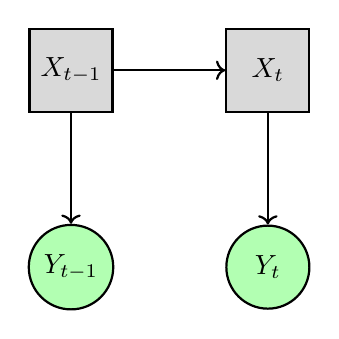
\begin{tikzpicture}[thick,node distance = {25mm},  state/.style = {draw, rectangle,fill= gray!30, minimum height=3em, minimum width=3em},
obs/.style = {draw, circle,fill= green!30, minimum height=3em, minimum width=3em}]
    
\node[state](1) {{$X_{t-1}$}};
    \node[state,right of=1](2) {{$X_t$}};
    \node[obs, below of=1](3) {{$Y_{t-1}$}};
    \node[obs, right of=3](4) {{$Y_{t}$}};
    \draw [->] (1) -- (2);
    \draw [->] (1) -- (3);
    \draw [->] (2) -- (4);
    
\end{tikzpicture}
\label{kal}
\caption{A Kalman filter described as a dynamic Bayesian network. The boxes represent the non observable state variables, and circles measurable data.}
\end{figure}

By exploiting the Markov property of the path from each node to the root of the tree, we can apply a Markov model of our choosing in analysing a whole sentence.
We will further exploit the fact that we can decide weather a sentence is parsed correctly only based on the tree produced, to split the model into two separate
parts. The first part will focus on analysing just the UD trees with a Markov model to produce the most probable parsings of a sentence. The other, which will for now depend heavily on the language under study, will give the probabilities for a word to be classified as a different part of speech based on its structure(for example, the english words ending with -ing can be either nouns or verbs). 


\clearpage
\subsection{Bare syntactic information}
For the purpose of analysing bare syntactic information, we propose Coupled Markov Model. This model we intuitively understand as most fittingly describing
the structure of the parse tree. We will assume that all states are observable, and that unconditional probabilities of all possible classifications are equal for both POS and syntactic relations. To train the model we will use sanitized datasets with language specific categories removed(which can be easily done in the CONLLu format). For now, we will only use data from one language(English) for training, but this can easily be extended to provide us with possible parse trees across hundreds of languages, and millions of sentences.
\begin{figure}[h!]
\center
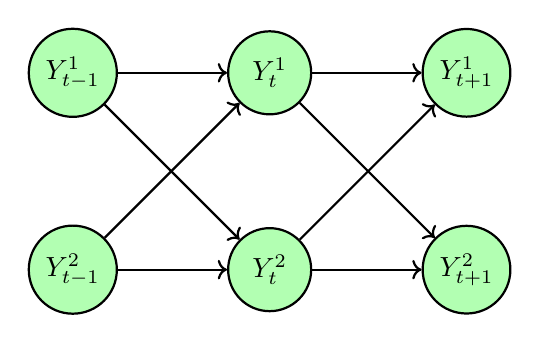
\begin{tikzpicture}[thick,node distance = {25mm},  state/.style = {draw, rectangle,fill= gray!30, minimum height=3em, minimum width=3em},
obs/.style = {draw, circle,fill= green!30, minimum height=3em, minimum width=3em}]
    
    \node[obs ](1) {{$Y_{t-1}^1$}};
    \node[obs, below of=1](2) {{$Y_{t-1}^2$}};

    \node[obs, right of=1](3) {{$Y_{t}^1$}};
    \node[obs, below of=3](4) {{$Y_{t}^2$}};

    \node[obs, right of=3](5) {{$Y_{t+1}^1$}};
    \node[obs, below of=5](6) {{$Y_{t+1}^2$}};


    \draw [->] (1) -- (3);
    \draw [->] (1) -- (4);

    \draw [->] (2) -- (3);
    \draw [->] (2) -- (4);
    
    \draw [->] (3) -- (5);
    \draw [->] (3) -- (6);

    \draw [->] (4) -- (5);
    \draw [->] (4) -- (6);
    
\end{tikzpicture}
\label{mark:synt}
\caption{Proposed complementary Markov model, with no hidden states representing the possible paths of a word to the root of the dependency tree}
\end{figure}
\subsection{Accounting for individual languages}
As mentioned before, we've had a lot of trouble in trying to find a universal way to extract grammatical information from a language. We are certain that
neural networks will be involved, but in order to use the training results across many languages, they have to be of a specific form. Since we aren't sure
what that form will be like, we will instead focus on interfacing with Markov Model. To this end, we propose a simple Recurrent neural network to classify
English words into its most probable POS tag and its syntactic relation to its head. This will require a lot of data, since there are a great many number of categories for each word, but since those are very regular, and we have a large dataset, we expect this task to not be very difficult. We can include it more directly
in our Markov model by having it provide us with an initial probability distribution for a given word.

\begin{figure}[h!]
\center
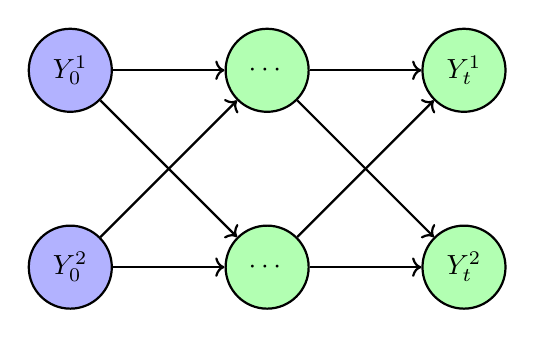
\begin{tikzpicture}[thick,node distance = {25mm},  state/.style = {draw, rectangle,fill= gray!30, minimum height=3em, minimum width=3em},
obs/.style = {draw, circle,fill= green!30, minimum height=3em, minimum width=3em}]
    
    \node[obs, fill=blue!30 ](1) {{$Y_{0}^1$}};
    \node[obs, fill=blue!30, below of=1](2) {{$Y_{0}^2$}};

    \node[obs, right of=1](3) {{$\cdots$}};
    \node[obs, below of=3](4) {{$\cdots$}};

    \node[obs, right of=3](5) {{$Y_{t}^1$}};
    \node[obs, below of=5](6) {{$Y_{t}^2$}};


    \draw [->] (1) -- (3);
    \draw [->] (1) -- (4);

    \draw [->] (2) -- (3);
    \draw [->] (2) -- (4);
    
    \draw [->] (3) -- (5);
    \draw [->] (3) -- (6);

    \draw [->] (4) -- (5);
    \draw [->] (4) -- (6);
    
\end{tikzpicture}
\label{mark:synt}
\caption{In this model, we assume that the initial probabilities for a given word(marked in blue), are provided by another model. This will change the probabilities of a word being tagged with a given POS tags, depending on the morphology of a word}
\end{figure}

One may think, that this breaks the Markov property, and in reality it does not, since we're using a Markov model only to generate possible paths to the root of the parse tree. The breaking of the Markov property will only occur once we try to combine those possible paths into a possible parse tree.
\clearpage

\subsection{Breakdown}
%    To summarize, the problem has been split into two separate problems. The first one being creating a language independent Markov model for UD parse trees. We assume that we can make it language independent by training it on parse trees from many different languages, which should train it to look for overarching grammatical structures across many different languages. One possible complication here, would be different sizes of tree banks. One could easily normalize circumvent this problem, by superimposing the Markov models over each other with different normalizing weights, but that issue will be dealt with once it appears.
%    The other being obtaining the initial probabilities. In training the model for obtaining these probabilities, we will assume that the only thing affecting them is the word itself, and not the other words in a sentence. We consider this a reasonable assumption, and expect those sentence wide relations to show up once combined with the Markov model. For the moment, this second problem will be interpreted as a simple classification problem, to be solved with a recurrent neural network. We will try to make the model as small as possible, and so will try to keep the network small.
%
To summarize, this chapter covered the use of the markov propperty between each node in the tree and its root in order to create a statistical "footprint" of a language. Since each language is different, each will have its own markov transition matrix that should produce the most likely paths through its syntax trees. Initialy, a word has a constant probability distribution in boths its classes. To create a more faithful model, these inital probabilities will be provided by a recurrent neural network described in the next chapter.
\subsubsection{Reality}
During implementation several issues turned up, which due to a lack of knowledge could not be remedied. The most important of which concerns the topology of the markov model. We've found no easily understood way to corelate the DEP and the POS transition matriecies in the split model, so a flattened model was used instead where each state is represented by a pair (POS,DEP).
This flattened model is very unwieldy, as it produces a sparse $666\times666$ matrix -- so sparse in fact that only 270 columns contain non--zero entries. It does however produce correct results, and even for large treebanks it can be calculated in a few minutes. This only has to be done once.
Regrettably however, despite the elegance of this approach, issues with the neural network precluded us from actualy putting it to use.



%\chapter{Serial chains}
\subsection{DHT parameters in biquaterionic form}
Denavit-Heartenberg convention can be used without modification with biquaternions instead of uniform matrices. If we write a transformation in the DHT convention as $a_i = r_{zi}t_{zi}r_{xi}t_{zi}$ then we'll have both:\\

\noindent  \begin{minipage}{0.5\linewidth}
\begin{equation}
    \begin{cases}
        r_{zi} = \cos{(\frac{\theta_i}{2})} + \sin{(\frac{\theta_i}{2})}k\\
        t_{zi} = 1 - \varepsilon \frac{d}{2} k\\
        r_{zi} = \cos{(\frac{\alpha_i}{2})} + \sin{(\frac{\alpha_i}{2})}i\\
        t_{zi} = 1 - \varepsilon\frac{a}{2} i 
    \end{cases}
\end{equation}    
\end{minipage}
\begin{minipage}{0.5\linewidth}

\begin{equation}
    \begin{cases}
        r_{zi}t_{zi} = \begin{bmatrix}
            R_z(\theta_i) &  \begin{bmatrix}
                0   \\ 0 \\ d
            \end{bmatrix} \\
                \mathbb{0} & 1
        \end{bmatrix}\\
        r_{xi}t_{xi} = \begin{bmatrix}
            R_x(\alpha) &  \begin{bmatrix}
                a   \\ 0 \\ 0
            \end{bmatrix} \\
                \mathbb{0} & 1
        \end{bmatrix}
    \end{cases}
\end{equation}    
\end{minipage}

One can check that these produce the same results. As an example a simple 2R manipulator will be described using biquaterionic DHT transformations.
\subsubsection{Example - 2R}
The DHT parameter table describing the 2R manipulator in its inital state is given below:
\begin{center}
\begin{tabular}{|c|c|c|c|c|}
\hline
i & $\theta_i$ & $d_i$ & $\alpha_i$ & $a_i$\\
\hline
1 & $\theta_1$ & 0 & 0 &  $L_1$ \\
\hline
2 & $\theta_2$ &0 &0 &  $L_2$\\
\hline
\end{tabular}
\end{center}
From this we get:
\begin{equation}
    \begin{cases}
        h_1 = (c_1+s_1k)(1-\frac{L_1}{2}\varepsilon i) = c_1+s_1k - \frac{L_1}{2}\varepsilon( c_1i+s_1j )\\
        h_2 = (c_2+s_2k)(1-\frac{L_2}{2}\varepsilon i) = c_2+s_2k - \frac{L_2}{2}\varepsilon( c_2i+s_2j )\\
    \end{cases}
\end{equation}
The last tranlation along the X axis can be actually skipped, but for the sake of consistancy it will be kept here.

\begin{equation}
    h = h_1h_2 = c_1c_2-s_1s_2 +
\end{equation}

\subsection{Plucker lines}

\subsection{Example - 2R manipulator}


%\chapter{November Milestone}
The goal of this project is to develop an algorithm for factoring a multivariate biquaterionic polynomial into factors corresponding to elementary
joints. For the november milestone the following subgoals have been acomplished:
\begin{enumerate}
        \item Describing serial chains using biquaterionic polynomials
        \item Development of a division algorithm for biquaterionic polynomials
        \item Initial investigation of the kinds of polynomials corresponding to mechanical joints in the multivariate case.
        
\end{enumerate}
As the first 2 subgoals were discussed in previous chapters, and as such will be covered briefly.
\section{Description of serial chains}
Although the Denavit-Heartenberg convention can be readily translated into
the language of biquaternions, it was found that it's more natural to use joint axes instead to describe the geometry of a given manipulator. 
While not a minimal description - the Denavit-Heartenberg convention is considered minimal as it reqieres only 4 parameters to describe a frame transforation - it gives insight into how a result of decomposition might look.
\\
As an ilutration, a planar 2R manipulator was described using linear
biquaterionic polynomials. The following motion polynomials
were obtained:
        \begin{equation}
            \begin{cases}
                R_1(t) = 1 + tk\\
                R_2(u) = (1-\varepsilon\frac{L_1}{2}i)(1+uk)(1+\varepsilon\frac{L_1}{2}) = 1+uk + u\varepsilon L_1j
            \end{cases}
        \end{equation}
        The product of which gives:
        \begin{equation}
           R(t,u)= R_1(t)R_2(u) = 1-tu +(t+u)k + \varepsilon L_1(sj-ti)
        \end{equation}
This bivariate motion polynomial can act on the end effector located at $1+\frac{\varepsilon}{2}(L_1+L_2)i$ for the initial configuration, producing:

   \begin{equation}
   \begin{cases}
        x' = 1 + \varepsilon\frac{Px\bar{P} + 2P\bar{Q}}{P\bar{P}}\\
        Px\bar{P} = (L_1+L_2)((1-ts)^2 - (s+t)^2)i+2(1-ts)(s+t)j\\
        P\bar{Q} = L_1(s^2-s t^2+s t+t)i + L_1(s^2 t+s t-s+t^2)j\\
        P\bar{P} = (1+t^2)(1+u^2)
   \end{cases}
   \end{equation}
After using the half-tangent identities to translate the result into the language of trigonometry the following forward kinematics were obtained:
   \begin{equation}
   \begin{aligned}
          x' = 1 &+ \varepsilon((L_1\cos{\theta_t} + L_2\cos{(\theta_t+\theta_u)})i\\
        &+(L_1\sin{\theta_t} + L_2\sin{(\theta_t+\theta_u)})j)
   \end{aligned}
   \end{equation}
Which are in agreement with ones found through other means.


\section{Division algorithm}
A division algorithm for multivariate polynomials requieres defning an ordering to its various monomial terms\cite{cox}. For a different ordering, different results will be obtained. Algorithms for a commutative field can be extended into the non-commutative case, by noting that there are now 2 division algorithms, a left and a right one. Both of these were described before, and were found to work as intended under the assumption that the indeterminates commute with the coefficients.
\\
\noindent\begin{minipage}{.5\linewidth}


\begin{algorithm}[H]
\KwIn{f1,f}
\KwOut{q,r}
\SetAlgoLined
\SetNoFillComment
\vspace{3mm}
$q \leftarrow 0; r \leftarrow 0$\\
$p \leftarrow f$\;
\While{p \neq 0}
{
    divisionoccured \leftarrow false\\
    \uIf{$LT(f_1)$ divides $LT(p)$}
    {
    $q \leftarrow q + LT(p) LT^{-1}(f_1)$\\
    $p \leftarrow p - LT(p) LT^{-1}(f_1)f_1$

    divisionoccured \leftarrow true\\
    }
    \uIf{ divisionoccured == false}
    {
        $r \leftarrow r + LT(p)$\\
         $p \leftarrow p - LT(p)$
   }
}
\Return q,r\;
\caption{Left division}
\end{algorithm}

\end{minipage}
\begin{minipage}{.5\linewidth}


\begin{algorithm}[H]
\KwIn{f1,f}
\KwOut{q,r}
\SetAlgoLined
\SetNoFillComment
\vspace{3mm}
$q \leftarrow 0; r \leftarrow 0$\\
$p \leftarrow f$\;
\While{p \neq 0}
{
    divisionoccured \leftarrow false\\
    \uIf{$LT(f_1)$ divides $LT(p)$}
    {
    $q \leftarrow q + LT^{-1}(f_1)  LT(p) $\\
    $p \leftarrow p -  f_1LT^{-1}(f_1) LT(p)$

    divisionoccured \leftarrow true\\
    }
    \uIf{ divisionoccured == false}
    {
        $r \leftarrow r + LT(p)$\\
         $p \leftarrow p - LT(p)$
   }
}
\Return q,r\;
\caption{Right division}
\end{algorithm}


\end{minipage}

As an example, the result of left division of the polynomial:
\begin{equation}
    f = 1 +ti + uj + tuk = (1 + ti)(1+uj)
\end{equation}
by $1+uh$ is:
\begin{equation}
    f= (1+uh)(th^{-1}k + h^{-1}j) + t(i - h^{-1}k) + 1 - h^{-1}j
\end{equation}
%%
Which has no remainder only if $h = j$

Something to keep in mind is that this remainder will be different depending on the chosen monomial ordering. This is concerning, as this gives the zeroing of the remainder as a sufficient, but not necessary condition for f1 to be a factor of f. For this algorithm to be useful then, one would need to find an appropriate order for agiven factor beforehand to zero its remainder. 


\section{Polynomial-joint correspondance}
This goal was not described previously, as it is still not fully entierly achieved. Before one can speak of a division algorithm, one should first know what he will divide into. Firstly, for a polynomial to correspond to a mechanical joint, it must not change its geometry depending on the values of the independant variables, as an example:
\begin{equation}
    H(t,u) = 1+\varepsilon( t i + u j)
\end{equation}
The above is a linear polynomial, which can not correspond to an elementary joint. Its geometry changes with the change of variables, which can't be the case for an elementary joint. This fact limits the polynomials which
can represent elementary joints to ones which can be described as:
\begin{equation}
    H(t_1,\dots,t_n) = 1 +R(t_1,t_2,\dots ,t_n)h
\end{equation}
Where $h \in \mathbb{DH}$ and $R \in \mathbb{R}[t_1,\dots ,t_n]$. Here the coefficient of h is a real polynomial, which represents for example how far a prismatic joint is extended, or a rotational joint rotated. But as there is only one biquaternion in the polynomial, the geometry stays the same.\\

Secondly, for a given decomposition, if we fix all variables but one, we should still have a viable closed loop kinematic chain capable of 1DOF motion. Consider:
\begin{equation}
    H(t_1,\dots,t_n) = (1+R_1(t_1,\dots,t_n)h_1)(1+R_2(t_1,\dots,t_n)h_2)
\end{equation}
If we fix all the variables except for $t_1$, we will get real polynomials in  $t_1$ as coefficients of biquaternions:

\begin{equation}
    H_{t_1}(t_1) = (1+(\Sigma_{i=0}^{m}a_it^{i}_1)h_1)(1+ (\Sigma_{i=0}^{m}b_it^{i}_1)h_2)
\end{equation}
If these polynomials contain quadratic terms, then we won't obtain a properly factored kinematic chain in 1 variable and would have to perform further divisions, which contradicts the fact that a factorised chain even existed. As such, after such an evaluation the coefficients must be linear:
\begin{equation}
    H_{t_1}(t_1) = (1+(a_0_a_1t)h_1)(1+ (b_0+b_1t)h_2)
\end{equation}

Furthermore, if we evaluate a given polynomial at 0 with all variables, we should get the identity polynomial, which implies that these coefficients have their 0 degree coefficients equal to 0.\\
Ultimately, a biquaterionic polynomial corresponds to a mechanical joint if it is of the form:
\begin{equation}
    H(t) = (1+ R(t_1,\dots,t_2)h)
\end{equation}
Where $R(t_1,\dots,t_2) \in R[t_1,\dots,t_n] / (t_1^{2},t_2^{2},\dots,t_n^{0})$, $R(0,\dots,0) = 0 $ and $h \in \mathbb{DH}$.  For the first 3 free variables, these polynomial coefficients would look as follows:s

\begin{equation}
    \begin{aligned}
        R(t)&=at&\mbox{1 free variable}\\[1.25ex]
        R(t,u)&= at + bu + ctu&\mbox{2 free variables}\\[1.25ex]
        R(t,u,v)&= at +bu + cv + dtu +etv +fuv +gtuv &\mbox{3 free variables}\\[1.25ex]
    \end{aligned}
\end{equation}

This immediatly implies that unlike for the univariate case, where a left evaluation would correspond to a left factor and vice versa, here we will have $n!$ left and right evaluations.
This is because once we evaluate this polynomial at a non-comutative element, the order in which they are multiplied matters. 
It is unclear at the moment, if the order of division would have any bearing on the propper order of evalation. 
It shouldn't since the division algorithm assumes that the free variables commue anyway, but it should be kept in mind that there may be some coupling there.

\section{December plans}
\begin{itemize}
        \item Under the assumption that joints correspond to the above derived factors, the conditions for factorization will be investigated.
        \item Behaviour of different orders of evaluation will be analysed.
        \item An attempt will be made to describe a serial parallel manipulator based on the human leg for further decomposition.
\end{itemize}


        


\chapter{Final report}

\section{Introduction}
To better explain the results of later chapters, quaternions and biquaternions are first introduced, along with their kinematic interpretations.
%% Biquaternions and biquaterionic polynomials



\subsection{Quaternions}
The algebra of quaternions -- usually denoted as $\mathbb{H}$ -- is homomorphic to the 3 dimensional special orthogonal group(SO(3)), which is the group representing rotations in 3D space. A general quaternion $h$ can be written as follows:
\begin{equation}
    h = h_0 + h_1i +h_2j + h_3k
\end{equation}
The 3 unit versors $i$,  $j$, $k$ are not commutative, and subject to the following equations:
\begin{equation}
       i^{2} = -1,\;
       j^{2} = -1,\;
       k^{2} = -1,\;
       ijk = -1
\end{equation}
A quaternion with its scalar par $h_0$ equal to zero is called a purely vectorial quaternion, the set of which is denoted as $\mathcal{H}$.  The conjugate of a quaternion is defined as:
\begin{equation}
    \bar{h} = h_0 - h_1i - h_2j - h_3k
\end{equation}
The conjugate can be used to define the square of the norm of a quaternion:
\begin{equation}
    h\bar{h} = \bar{h}h = h_0^{2} + h_1^{2}+h_2^{2} + h_3^{2} \in \mathbb{R}
\end{equation}
If $h \in \mathcal{H}$, then $h + \bar{h} = 0$.
\clearpage
\subsubsection{SO(3)}
Given $v \in \mathcal{H}$, a quaternion $p \in \mathbb{H}$ can be used to rotate it around the origin by the following map:
\begin{equation}
    v' = \frac{pv\bar{p}}{p\bar{p}}
\end{equation}
In particular, if $p$ is a unit quaternion with $p\bar{p} = 1$ we have:

\begin{equation}
    v' = pv\bar{p}
\end{equation}
This is sometimes affectionately referred to as the \textbf{sandwich product}.
\\
To understand how a sandwich product of a quaternion $p$ rotates $v$, it helps to observe, that every unit quaternion can be written as:
\begin{equation}
    p = \cos{(\frac{\theta}{2})} + \sin{(\frac{\theta}{2})}u
\end{equation}
where $u\bar{u} = 1$ and  $u\in \mathcal{H}$. Then the sandwich product represents rotation of $v$ around the axis $u$ by the angle $\theta$.
To convince ourselves of this, we can first see that a rotation of $u$ around $u$ leads to the identity transformation, and investigate the behaviour of unit versors.\\
\subsubsection{Rotation of a versor lying on the rotation axis}
\begin{equation}
    \begin{aligned}
        u'&=pv\bar{p}&\mbox{}\\[1.25ex]
        u'&=(\cos{(\frac{\theta}{2})}+\sin{(\frac{\theta}{2})u})u(\cos{(\frac{\theta}{2})}-\sin{(\frac{\theta}{2})u})&\mbox{}\\[1.25ex]
        u'&=(\cos{(\frac{\theta}{2})}+\sin{(\frac{\theta}{2})u})(\cos{(\frac{\theta}{2})}u+\sin{(\frac{\theta}{2})})&\mbox{}\\[1.25ex]
        u'&=(\cos{(\frac{\theta}{2})}^{2} + \sin{(\frac{\theta}{2})}^{2})u&\mbox{}\\[1.25ex]
        u'&=u&\mbox{}\\[1.25ex]
    \end{aligned}
\end{equation}
\subsubsection{Rotation of a basis versor around another basis versor}
Let $p = \cos{(\frac{\theta}{2})} + \sin{(\frac{\theta}{2})}k$, then if we calculate the sandwich products $pi\bar{p}$ or  $pj\bar{p}$ we should expect results similar to ones well known from linear algebra:\\

\noindent\begin{minipage}{.5\linewidth}
    \begin{equation}
        \begin{bmatrix}
            \cos{(\theta)} \\
            \sin{(\theta)} \\
            0
        \end{bmatrix} = \begin{bmatrix}
        \cos{(\theta)} & -\sin{(\theta)} & 0\\
        \sin{(\theta)} & \cos{(\theta)} & 0 \\
        0 & 0 & 1
        \end{bmatrix}
        \begin{bmatrix}
            1  \\ 0 \\ 0
        \end{bmatrix}
    \end{equation}
\end{minipage}
\begin{minipage}{.5\linewidth}
    \begin{equation}
             \begin{bmatrix}
            -\sin{(\theta)} \\
            \cos{(\theta)} \\
            0
        \end{bmatrix} = \begin{bmatrix}
        \cos{(\theta)} & -\sin{(\theta)} & 0\\
        \sin{(\theta)} & \cos{(\theta)} & 0\\
        0 & 0 & 1
        \end{bmatrix}
        \begin{bmatrix}
            0  \\ 1 \\ 0
        \end{bmatrix}
    \end{equation}
\end{minipage}
And in fact:
\begin{equation}
    \begin{aligned}
         u'&=pi\bar{p}&\mbox{}\\[1.25ex]
        u'&=(\cos{(\frac{\theta}{2})}+\sin{(\frac{\theta}{2})k})i(\cos{(\frac{\theta}{2})}-\sin{(\frac{\theta}{2})k})&\mbox{}\\[1.25ex]
        u'&=(\cos{(\frac{\theta}{2})}+\sin{(\frac{\theta}{2})k})(\cos{(\frac{\theta}{2})}i+\sin{(\frac{\theta}{2})}j)&\mbox{}\\[1.25ex]
        u'&=(\cos{(\frac{\theta}{2})}^{2}-\sin{(\frac{\theta}{2})}^{2})i + 2\sin{(\frac{\theta}{2})}\cos{(\frac{\theta}{2})}j&\mbox{}\\[1.25ex]
        u'&=\cos{(\theta)}i + \sin{(\theta})j&\mbox{}\\[1.25ex]

    \end{aligned}
\end{equation}
A result in complete agreement with one obtained by the use of rotation matrices

\clearpage

\subsubsection{T(3)}

Since we already associate the 3 basis versors with the 3 standard axes of a Cartesian space, it seems natural to use quaternions to represent translations. It is in fact trivial to do, a translation is simply the addition of one purely vectorial quaternion to another:
\begin{equation}
    v' = v + u
\end{equation}
where $v,u\in \mathcal{H}$.
\subsubsection{SE(3)}
The special Euclidean group(SE(3)), which represents rigid body motions in 3D space, is composed of 2 subgroups. Those being the special orthogonal group SO(3), and the translational group in 3D T(3). Given these 2, one can construct SE(3) as the semi-direct product of them as such:
\begin{equation}
    SE(3) = SO(3)\ltimes T(3)
\end{equation}
With this construction, elements of SE(3) are given by a tuple  $(r,t)$, and a product of 2 of its elements is given as follows:
 \begin{equation}
     \label{semidirect}
     (r_2,t_2)(r_1,t_1) = (r_2r_1,r_2t_1\bar{r}_2+t_2)
\end{equation}
With $r_1,r_2\in SO(3)$, and $t_1,t_2 \in T(3)$\\
This formula should be familiar to anyone who ever multiplied 2 DHT matrices together.\\
In general then, a pair of quaternions is enough to represent the motion of rigid bodies. A problem however with this formulation is that it requires pairs of quaternions, which makes it mathematically unwieldy. This leads to the idea of enclosing both of these pairs in a single algebra.
\subsection{Biquaternions}
The way the above issue can be solved when using orthogonal matrices to represent rotation, is to embed SE(3) in SO(4). This may sound complicated, but this is in fact the most common way to represent elements of SE(3). An example would be the block matrix:
\begin{equation}
    A_i = \begin{bmatrix}
        R & T   \\
        \mathbb{0} & 1
    \end{bmatrix}
\end{equation}
Again, this should be familiar to anyone who knows anything about robot kinematics. If we multiply 2 such matrices together we will obtain:
\begin{equation}
    A_1A_2 =  \begin{bmatrix}
        R_1 & T_1   \\
        \mathbb{0} & 1
    \end{bmatrix} 
 \begin{bmatrix}
        R_2 & T_2   \\
        \mathbb{0} & 1
    \end{bmatrix} 
 \begin{bmatrix}
        R_1R_2 & R_2T_1 + T_2\\
        \mathbb{0} & 1
    \end{bmatrix}
\end{equation}
Which looks exactly like the semi-direct product presented before \ref{semidirect}. Do tho this with quaternions however, we have to utilise a different method. A way to do this, is to introduce a new type of coefficient for 
regular quaternions. Instead of using real numbers $h_i \in \mathbb{R}$ as coefficients, one can introduce dual number coefficients $h_i \in \mathbb{D}$ $h_i = p_i + \varepsilon q_i$, where  $\varepsilon^{2} = 0$. By using these dual coefficients, we create a new algebra called the dual quaternions(sometimes also known as bi quaternions) which we will denote as $\mathbb{DH}$. An element $h \in \mathbb{DH}$ can also be written as 
 \begin{equation}
    h = p + \varepsilon q
\end{equation}
Where $p,q \in \mathbb{H}$. 
A necessary condition for a biquaternion to describe an element of SE(3) is that it lies in the Study quadric\cite{Heged_s_2013}. This condition for a biquaternion can be alternatively stated that it needs to have a real non-zero norm. A norm of a biquaternion is defined in terms of its conjugate as follows:
\begin{equation}
    \begin{aligned}
        h\bar{h}=(p+\varepsilon q)\bar{(p+\varepsilon q)}\\
        h\bar{h}=(p+\varepsilon q)(\bar{p}+\varepsilon \bar{q})\\
        h\bar{h}=p\bar{p} + \varepsilon (p\bar{q} + q\bar{p}) 
    \end{aligned}
\end{equation}
For the above to be a real number, the dual part needs to be zero, e.g. $  (p\bar{q} + q\bar{p}) = 0$. The rotation can be extracted by just taking the primal part p of the biquaternion. Its action upon elements of SE(3) is defined the same as for regular quaternions. The position of a point in space - represented as $x = 1+\varepsilon v$, where v is a vectorial quaternion - is given by the map\cite{Siegele_2021}:
\begin{equation}
     x \rightarrow \frac{(p - \epsilon q)x(\bar{p}+\epsilon \bar{q})}{p\bar{p}}
\end{equation}
Which can be rewritten:
\begin{equation}
    \label{act}
    \begin{aligned}
        \frac{(p - \epsilon q)x(\bar{p}+\epsilon \bar{q})}{p\bar{p}}&=\frac{px\bar{p} + \epsilon(px\bar{q} - qx\bar{p})}{p\bar{p}}&\\[1.25ex]
        \frac{px\bar{p} + \epsilon(px\bar{q} - qx\bar{p})}{p\bar{p}}&= 1+\epsilon\frac{pv\bar{p} + p\bar{q} - q\bar{p}}{p\bar{p}}&\\[1.25ex]
        1+\epsilon\frac{pv\bar{p} + p\bar{q} - q\bar{p}}{p\bar{p}}&= 1 + \epsilon \frac{pv\bar{p} + 2p\bar{q}}{p\bar{p}}&\\[1.25ex]
    \end{aligned}
\end{equation}

Note that the map does not require the biquaternion to be of unit norm. In fact, the mapped point remains the same no matter what real number we multiply the polynomial by. By noticing this, we can treat the space of rigid body motions as a projective space, allowing for the use of polynomials to represent trajectories in it. The simplest such motions are translations along a line, and rotation around a point. Both can be described using linear biquaterionic polynomials.

\subsubsection{Elementary motions}
A linear biquaterionic polynomial can represent either a translation, or a rotation. 
A general formula for a linear univariate biquaterionic polynomial parametrising a rigid body motion is the following:
\begin{equation}
    F = 1+th,\; h \in \mathbb{DH}
\end{equation}
To represent a motion in SE(3), its norm polynomial has to be real:
\begin{equation}
    F\bar{F} = 1+(h+\bar{h})t+h\bar{h}t^{2} \in \mathbb{R}[t]
\end{equation}
Since the parameter t is always real, this translates to:
\begin{equation}
    \begin{cases}
        h\bar{h} \in \mathbb{R}\\
        h+\bar{h} \in \mathbb{R}
    \end{cases}
\end{equation}
Since $h = p + \epsilon q,\; p,q \in \mathbb{H}$, this is equivalent to saying that $h$ itself has to satisfy the Study condition -- and so represent an element of SE(3) -- and has to have purely vectorial dual part, e.g.
\begin{equation}
    h = p_0+p_1\mathit{i}+p_2\mathit{j}+p_3\mathit{k} +\epsilon(q_1\mathit{i}+q_2\mathit{j}+q_3\mathit{k})
\end{equation}
\subsubsection{Elementary motions -- translation}
Translations form a subgroup of SE(3), and can be easily represented by a purely dual biquaternion. In general such a quaternion has the form:
\begin{equation}
    h_t = 1 - \frac{\epsilon}{2}(q_1\mathit{i}+q_2\mathit{j}+q_3\mathit{k})
\end{equation}
Its action will translate a given point $x = 1 + \epsilon(v)$ along the vector $q$ according to \ref{act}:
\begin{equation}
    \begin{aligned}
        x &\rightarrow 1 + \epsilon\frac{pv\bar{p} + 2p\bar{q}}{p\bar{p}}&\mbox{Note that $p = 1$ and  $q = q_1\mathit{i}+q_2\mathit{j}+q_3\mathit{k}$}\\[1.25ex]
        x&\rightarrow 1 + \epsilon(v + q)&\mbox{The point is mapped onto its original position plus the translation vector}\\[1.25ex]
    \end{aligned}
\end{equation}

We can parametrise this map using a real parameter $t$, thus giving rise to a linear biquaterionic polynomial parametrisation of translations in SE(3):
\begin{equation}
    H_t(t) = 1 - \frac{\epsilon t}{2}q
\end{equation}
It maps a point x -- defined as before -- as follows:
\begin{equation}
    x \rightarrow  1 + \epsilon v + \epsilon qt
\end{equation}
The parameter t specifies where along the line defined by the vector q the point is translated. For $t = 0$ we get the identity transformation.
Since $h_t$ satisfies the Study condition, so does  $H_t$, and thus we've associated translations with linear trajectories in the study quadric.
\subsubsection{Elementary motions -- rotations}
It is well known, that rotations around the origin can be represented by unit quaternions. This representation can easily be extended to the projective case, and gives an intuitive interpretation of the indeterminate parametrising the rotation. A quaternion representing a rotation about an axis $q$ located at the origin is given by the following:
\begin{equation}
    \begin{aligned}
        q&= \cos{\theta} + \sin{\theta}(q_1\mathit{i} + q_2\mathit{j} + q_3\mathit{k})&\mbox{Divide by $\cos{\theta}$}\\[1.25ex]
        \frac{q}{\cos{\theta}}&\equiv q&\mbox{$\equiv$ we take to mean projectively equal}\\[1.25ex]
        q&\equiv 1 + \tan{\theta}(q_1\mathit{i} + q_2\mathit{j} + q_3\mathit{k})&\mbox{}\\[1.25ex]
    \end{aligned}
\end{equation}
By interpreting $\tan{\theta}$ as the indeterminate variable t, we can represent rotation around an axis at the origin as a linear quaterionic polynomial. \\
To represent a rotation around an axis located at another location, the translation biquaternion can be used to translate the rotation quaternion\cite{Siegele_2021}. To do this, the same map \ref{act} as the one used to represent the movement of a point can be used, but instead of a point it will act on a rotation quaternion. 
\begin{equation}
    \label{rottr}
    \begin{aligned}
        (1-\epsilon \frac{x}{2})(1+tv)(1+\epsilon \frac{x}{2}))   &= 1 + tv +t\frac{\epsilon}{2}(vx-xv)&\mbox{}\\[1.25ex]
        P(t)&= 1 + tv&\mbox{The primal part}\\[1.25ex]
        Q(t)&= \frac{t}{2}(vx-xv)&\mbox{The dual part}\\[1.25ex]
    \end{aligned}
\end{equation}
The above map describes a rotation around an axis $v$, which goes through a point $x$. To see that this is the case, we can show that it's action is not going to affect any point which lies on the axis it rotates around. The coordinates of all such unaffected points will lie on a line which can be represented as a biquaternion $z = 1 + \epsilon(x + u v)$, where  $u\in \mathbb{R}$, and both x and v are purely vectorial quaternions, with $v\bar{v} = 1$. Then the point $z$ will be mapped to another point by \ref{rottr} according to \ref{act}:
\begin{equation}
    z \rightarrow 1 +\epsilon \frac{P(t)(x+uv)P(t) + 2P(t)\bar{Q}(t)}{P(t)\bar{P}(t)}
\end{equation}
The second part can be expanded as:
\begin{equation}
    \begin{aligned}
        2P(t)\bar{Q}(t)&=2(1+tv)\frac{t}{2}(xv-vx)&\mbox{}\\[1.25ex]
        2P(t)\bar{Q}(t)&=t(xv-vx)+t^{2}(vxv - x)&\mbox{}\\[1.25ex]
    \end{aligned}
\end{equation}
While the first as:
\begin{equation}
    \begin{aligned}
        P(t)(x+uv)P(t)&=P(t)x\bar{P}(t) + u P(t)v\bar{P}(t)&\mbox{}\\[1.25ex]
        uP(t)v\bar{P}(t)&= u(1+t^{2})v&\mbox{}\\[1.25ex]
        P(t)x\bar{P}(t)&= x + t(vx-xv)-t^{2}vxv&\mbox{}\\[1.25ex]
    \end{aligned}
\end{equation}

Adding both of these together we get:
\begin{equation}
    P(t)(x+uv)\bar{P}(t) + 2P(t)\bar{Q}(t) = x + t(vx-xv) - t^{2}vxv+u(1+t^{2}) + t(xv-vx) + t^{2}(vxv-x)
\end{equation}
Which after simplification yields:
\begin{equation}
    P(t)(x+uv)\bar{P}(t) + 2P(t)\bar{Q}(t) = (x + uv)(1+t^{2})
\end{equation}
Which ultimately shows that this rotation polynomial maps z to itself:
\begin{equation}
    z \rightarrow 1+\epsilon(x+uv)
\end{equation}

\subsection{Bivariate polynomials}
Extending this to the bivariate case, there are a couple of possibilities as to what will serve as the analogue of the linear elementary motions. For a serial chain with every joint being independent, there is no such problem, and we can simply take the new linear terms to be in either of the free variables. This assumption simplifies calculations by a large margin, but restricts the class of motion polynomials under consideration to those who's norm can be written as a product of 2 polynomials in 2 different variables. This latter approach was ultimately the one chosen, however a discussion of the alternative choice will follow later on in the report.\\
We are now in a position to state the design procedure.
\begin{itemize}
    \item Describe a desired 2 DOF motion using a motion polynomial. This serves as an analogue to the virtual chain of Dr Gosselin's method\cite{gosselin}.
    \item Factorize this motion polynomial, to produce the following representation:
        \begin{equation}
    H(u,t) = (1-h_0 v_0)(1-h_1 v_1)\dots(1-h_nv_n)
        \end{equation}
Where:
\begin{itemize}
        \item $h_i$ - is a motion biquaternion describing a rotation
        \item  $v_i \in \left\{ u, t \right\}$ - is a free variable taking on real values       
\end{itemize}
There may be multiple such factorizations, each of which represents a serial kinematic chain realising the desired motion.
\item Somehow constrain these chains to restrict the degrees of freedom of each mechanism to the number of free variables in the motion polynomial. Thus creating the desired mechanism.
\end{itemize}


\section{Methods}
Despite the assumed simplifications, the problem is still very complex.
To simplify computations, another simplification was made based on the observation, that every motion in $SE(3)$ has a spherical projection in  $SO(3)$. This is because rotation is not changed by a translation, so for example a 6 DOF manipulator may be performing very complex motions, the orientation of the end effector is just the result of multiplying individual joint rotation matrices. 
This means, that every spatial mechanism can be reduced to a spherical one containing only rotation, and that a spherical mechanism can be turned into a spatial one by translating its rotation axes.\\
In case of biquaterionic polynomials, this means that just the product of
the quaterionic parts of every polynomial defines a spherical mechanism. What's more its decomposition will be the same as the spatial one if one removes the dual part from every term in the product. To illustrate this process, a motion polynomial describing the spatial motion of a Bennet mechanism is considered\cite{li2015factorization} :
\begin{equation}
    C(t) = 1 +  (1-j)t + (1-i-j-k)t^{2} - \varepsilon((i-j-k)t-(1+k)t^{2})
\end{equation}
This mechanism admits 2 factorizations:
\begin{equation}
    \begin{cases}
        C(t) = (1-t(j+k+\varepsilon(i+j-k)))(1+t(1+k+2\varepsilon j ))\\
        C(t) = (1+t(1+i+\varepsilon k))(1-t(i+j+\varepsilon(i-j))
    \end{cases}
\end{equation}
The spherical projection is obtained by taking the real part of each factor, and the result is the real part of $C(t)$, which is a viable quaterionic motion polynomial, and as such represents a spherical mechanism.

\begin{equation}
    PrimalPart(C(t)) = 1 +  (1-j)t + (1-i-j-k)t^{2}
\end{equation}
This mechanism admits 2 factorizations:
\begin{equation}
    \begin{cases}
        PrimalPart(C(t)) = (1-t(j+k))(1+t(1+k))\\
        PrimalPart(C(t)) = (1+t(1+i+k))(1-t(i+j))
    \end{cases}
\end{equation}
This ultimately means, that as long as this method works for quaterionic polynomials, it will work for biquaterionic ones as well.

\subsection{Desired motion}
The motion polynomial considered was designed to rotate the z axis to a position described by spherical coordinates:
\begin{equation}
    qk\bar{q} \rightarrow i \sin{\theta}\cos{\psi}  +  j \sin{\theta}\sin{\psi}  + k\cos{\theta}
\end{equation}

\begin{figure}[h!]
    \centering
    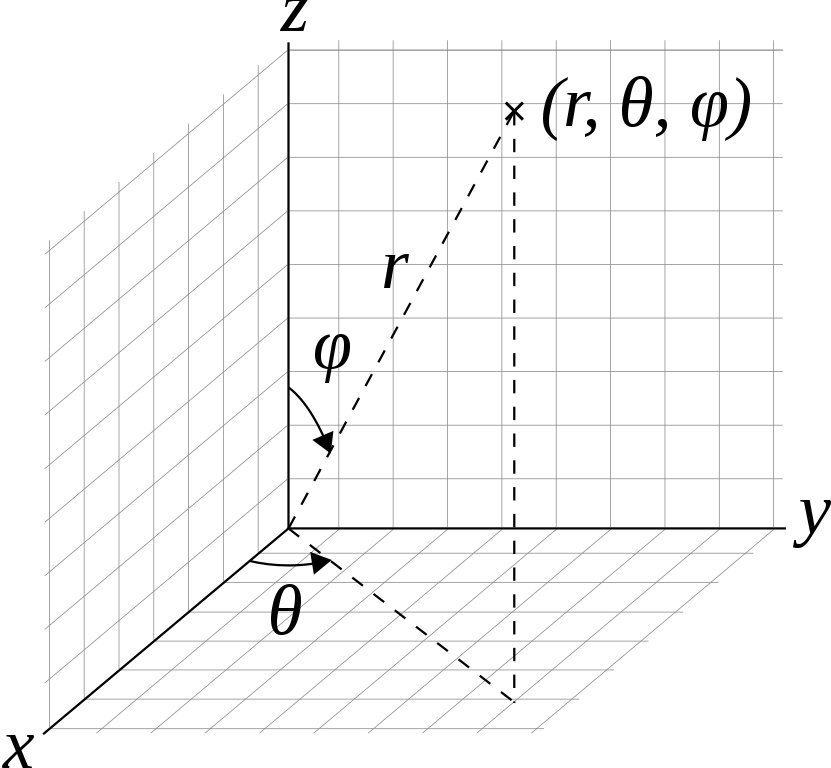
\includegraphics[scale=0.3]{img/831px-3D_Spherical_2.png}
    \caption{Visualisation of the \href{  https://en.wikipedia.org/wiki/Spherical_coordinate_system }{spherical coordinate frame} in relation to the cartesian one.}
    \label{fig:enter-label}
\end{figure}

There is no one single way to find a polynomial transforming one vector into the other. A way to do it involves finding the vector cross product of the 2 vectors - say $v$ and  $u$ - to represent the rotation axis, and their dot product to determine the angle of rotation:
\begin{equation}
    q = v\cdot u + \sqrt{u\bar{u}v\bar{v}} + v \times u
\end{equation}
Applying this method to the 2 vectors in the map given at the beginning we obtain:
\begin{equation}
    q = 1 + \cos{\theta} + \sin{\theta}(\cos{\psi}j-\sin{\psi}i)
\end{equation}
This polynomial does not have unit norm, but does describe the correct rotation.
We can projectivise it by using the half tangent formulas for the trigonometric functions. Since this is all in a projective space, the motion polynomial can be multiplied by any scalar - in this case its norm polynomial - and still produce the same motion.
\begin{equation}
    C(u,t) = 1+u^{2}-2tui - t(u^{2}-1)j
\end{equation}
This is the polynomial who's properties are investigated in the remainder of this report. 
\section{Results}
In order to better visualise the procedure being followed, a network will be used to describe the sequence of transformations from one link to another. This is similar to how voltages are described in an electrical network.
First the overall transformation can be described as such:

\begin{figure}[h!]
\begin{center}
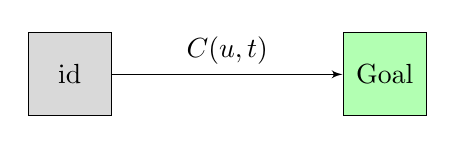
\begin{tikzpicture}[block/.style = {draw, fill=white, rectangle, minimum height=3em, minimum width=3em},
sum/.style= {draw, fill=white, circle, node distance=1cm},
input/.style = {coordinate},
tmp/.style = {coordinate},
output/.style= {coordinate},
pinstyle/.style = {pin edge={to-,thin,black}},
auto,
node distance = 2cm,
>=latex'
]


    \node [block, fill=gray!30] (id) {id};
    \node [block, right of=id, fill=green!30, node distance=4cm] (end) {Goal};

    \draw [->] (id) -- node{$C(u,t)$}(end);

\end{tikzpicture}
\caption{The origin is colored gray, and effector transformation is colored green.}
\label{}
\end{center}
\end{figure}
The transformation between 2 vertices is given by the previously described map \ref{act}(this map also works for quaternions). By factorising, we will obtain an equivalent transformation sequence, which is directly realisable mechanically using elementary joints. This can be symbolically described as follows:

\begin{figure}[h!]
\begin{center}
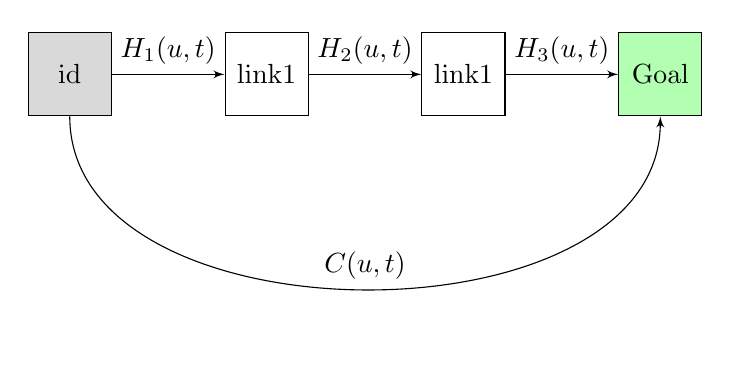
\begin{tikzpicture}[block/.style = {draw, fill=white, rectangle, minimum height=3em, minimum width=3em, node distance=2.5cm},
sum/.style= {draw, fill=white, circle, node distance=1cm},
input/.style = {coordinate},
tmp/.style = {coordinate},
output/.style= {coordinate},
pinstyle/.style = {pin edge={to-,thin,black}},
auto,
node distance = 2cm,
>=latex'
]


    \node [block, fill=gray!30] (id) {id};
    \node [block,right of=id] (link1) {link1};
    \node [block,right of=link1] (link2) {link1};
    \node [block, right of=link2, fill=green!30, node distance=2.5cm] (end) {Goal};

    \draw [->] (id) -- node{$H_1(u,t)$}(link1);
    \draw [->] (link1) -- node{$H_2(u,t)$}(link2);
    \draw [->] (link2) -- node{$H_3(u,t)$}(end);

    \draw [->] (id) to [out=-90,in=-90] node{$C(u,t)$}(end);

\end{tikzpicture}
\caption{The 2 paths to the goal would describe the same motion by construction}
\label{}
\end{center}
\end{figure}

The factorization methods for multivariate biquaterionic polynomials are still in their infancy\cite{ lercher2021multiplication, Lercher_2022 }. The methods used for the univariate case are more developed, but break down in the multivariate case quite spectacularly, producing factors which change their geometry during movement. However, as this is a very simple case, the factorization can be done by hand manually producing the following factorization:
\begin{equation}
    C(u,t) = (1+uk)(1+jt)(1-uk)
\end{equation}
This factorization is interesting, as it can be thought of as a rotation around the y axis, which is first rotated around the z axis. 
The first problem here is that this is a 3R chain which is supposed to perform a 2DOF motion. For that to be the case the movement has to be constrained. In the univariate case this is done by connecting multiple factorizations of the same movement  to the end effector. If described using a diagram it would look like this:

\begin{figure}[h!]
\begin{center}
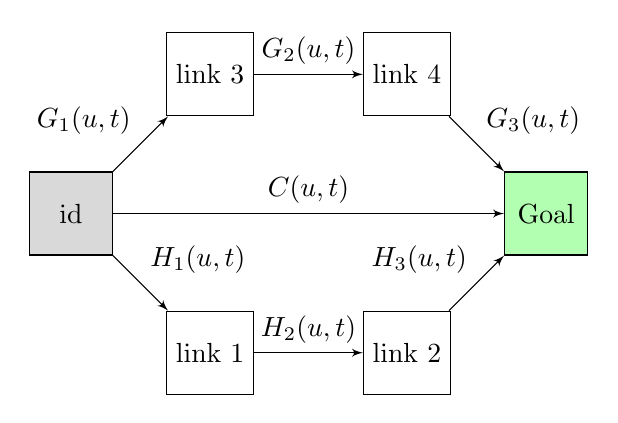
\begin{tikzpicture}[block/.style = {draw, fill=white, rectangle, minimum height=3em, minimum width=3em, node distance=2.5cm},
sum/.style= {draw, fill=white, circle, node distance=1cm},
input/.style = {coordinate},
tmp/.style = {coordinate},
output/.style= {coordinate},
pinstyle/.style = {pin edge={to-,thin,black}},
auto,
node distance = 2cm,
>=latex'
]


    \node [block, fill=gray!30] (id) {id};
    \node [block,below right of=id] (link1) {link 1};
    \node [block,right of=link1] (link2) {link 2};
    \node [block,above right of=id] (link3) {link 3};
    \node [block,right of=link3] (link4) {link 4};
    \node [block, above right of=link2, fill=green!30, node distance=2.5cm] (end) {Goal};

    \draw [->] (id) -- node{$H_1(u,t)$}(link1);
    \draw [->] (link1) -- node{$H_2(u,t)$}(link2);
    \draw [->] (link2) -- node{$H_3(u,t)$}(end);

    \draw [->] (id) -- node{$G_1(u,t)$}(link3);
    \draw [->] (link3) -- node{$G_2(u,t)$}(link4);
    \draw [->] (link4) -- node{$G_3(u,t)$}(end);

    \draw [->] (id) -- node{$C(u,t)$}(end);

\end{tikzpicture}
\caption{A hypothetical alternate factorization}
\label{}
\end{center}
\end{figure}



Here however that is impossible, as it was found that no other factorization exists. Not to mention, even if it were possible, another constraint would have to be imposed on the mechanism in the form of another loop. This is because according to the mobility formula for spherical mechanisms:
\begin{equation}
    M = J - 3L
\end{equation}
Where J is the number of joints of the mechanism, and L the number of independent loop closure conditions, the mobility of such mechanism would be 3, not 2. Usually these kinds of parallel mechanisms have 3 joints in one arm, and 2 in the other. This way only one loop is needed. It is unclear at the moment how such a factorization could be created, but it would necessitate a different form of the factor representing elementary motions. \\
Another approach was tried, where an artificial scaffolding would be constructed around the main mechanism, which would create the necessary constraints. There are 2 possible topologies for such a scaffold:
\begin{figure}[h!]
\begin{center}
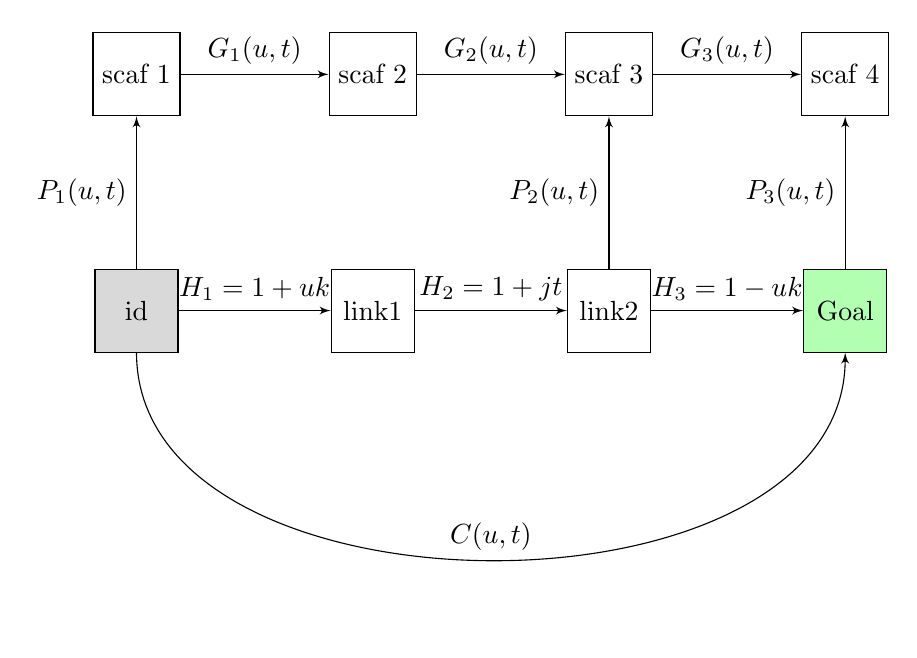
\begin{tikzpicture}[block/.style = {draw, fill=white, rectangle, minimum height=3em, minimum width=3em, node distance=3cm},
sum/.style= {draw, fill=white, circle, node distance=1cm},
input/.style = {coordinate},
tmp/.style = {coordinate},
output/.style= {coordinate},
pinstyle/.style = {pin edge={to-,thin,black}},
auto,
node distance = 2cm,
>=latex'
]


    \node [block, fill=gray!30] (id) {id};
    \node [block,right of=id] (link1) {link1};
    \node [block,right of=link1] (link2) {link2};
    \node [block, right of=link2, fill=green!30, node distance=3cm] (end) {Goal};

    \node [block, above of=id] (ids) {scaf 1};
    \node [block,right of=ids] (link1s) {scaf 2};
    \node [block,right of=link1s] (link2s) {scaf 3};
    \node [block, right of=link2s, node distance=3cm] (ends) {scaf 4};




    \draw [->] (id) -- node{$P_1(u,t)$}(ids);
    \draw [->] (link2) -- node{$P_2(u,t)$}(link2s);
    \draw [->] (end) -- node{$P_3(u,t)$}(ends);

    \draw [->] (id) -- node{$H_1 = 1+uk$}(link1);
    \draw [->] (link1) -- node{$H_2 = 1+jt$}(link2);
    \draw [->] (link2) -- node{$H_3 = 1-uk$}(end);

    \draw [->] (ids) -- node{$G_1(u,t)$}(link1s);
    \draw [->] (link1s) -- node{$G_2(u,t)$}(link2s);
    \draw [->] (link2s) -- node{$G_3(u,t)$}(ends);

    \draw [->] (id) to [out=-90,in=-90] node{$C(u,t)$}(end);

\end{tikzpicture}
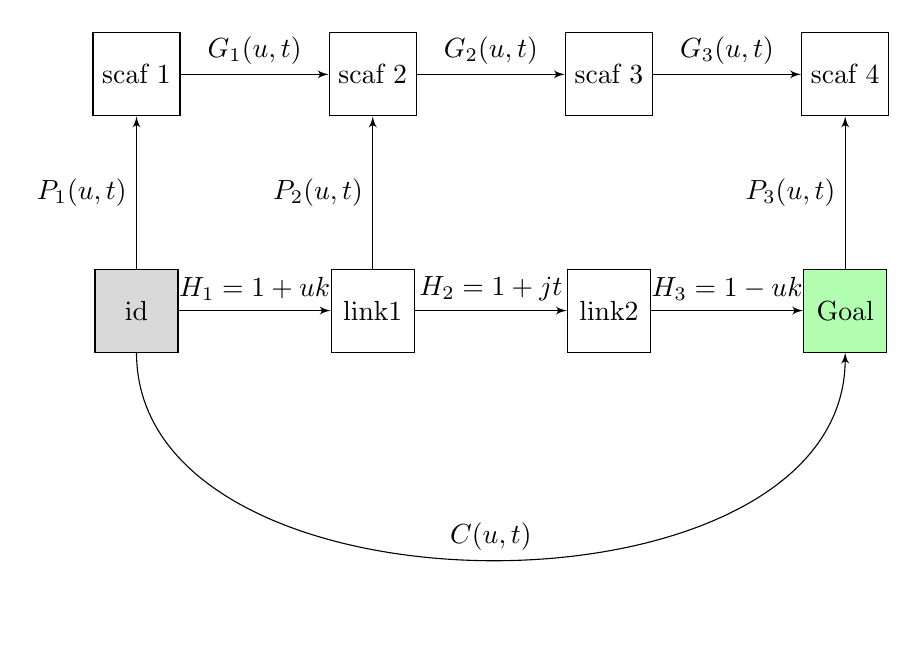
\begin{tikzpicture}[block/.style = {draw, fill=white, rectangle, minimum height=3em, minimum width=3em, node distance=3cm},
sum/.style= {draw, fill=white, circle, node distance=1cm},
input/.style = {coordinate},
tmp/.style = {coordinate},
output/.style= {coordinate},
pinstyle/.style = {pin edge={to-,thin,black}},
auto,
node distance = 2cm,
>=latex'
]


    \node [block, fill=gray!30] (id) {id};
    \node [block,right of=id] (link1) {link1};
    \node [block,right of=link1] (link2) {link2};
    \node [block, right of=link2, fill=green!30, node distance=3cm] (end) {Goal};

    \node [block, above of=id] (ids) {scaf 1};
    \node [block,right of=ids] (link1s) {scaf 2};
    \node [block,right of=link1s] (link2s) {scaf 3};
    \node [block, right of=link2s, node distance=3cm] (ends) {scaf 4};




    \draw [->] (id) -- node{$P_1(u,t)$}(ids);
    \draw [->] (link1) -- node{$P_2(u,t)$}(link1s);
    \draw [->] (end) -- node{$P_3(u,t)$}(ends);

    \draw [->] (id) -- node{$H_1 = 1+uk$}(link1);
    \draw [->] (link1) -- node{$H_2 = 1+jt$}(link2);
    \draw [->] (link2) -- node{$H_3 = 1-uk$}(end);

    \draw [->] (ids) -- node{$G_1(u,t)$}(link1s);
    \draw [->] (link1s) -- node{$G_2(u,t)$}(link2s);
    \draw [->] (link2s) -- node{$G_3(u,t)$}(ends);

    \draw [->] (id) to [out=-90,in=-90] node{$C(u,t)$}(end);

\end{tikzpicture}
\caption{Second scaffold creates a 4 bar near the base of the mechanism, whle the first near the end}
\label{}
\end{center}
\end{figure}

\clearpage
The polynomial $P_2$ can be more or less chosen arbitrarily. It was chosen however, to make the 4 bars univariate. In each of these topologies, there are 3 ways to choose the factors, giving 6 cases to consider. Regrettably, none of these cases produced a viable mechanism. 
\\
Finally, to determine where it all went wrong, an attempt was made to analyse an actual 2DOF spherical manipulator using this method. The manipulator chosen was a simplified version of the 3DOF "Agile Eye" manipulator developed by dr. Gosselin . 
A system of equations was developed based on the description of how the passive joint angles depend on the 2 active ones. It was found that its solution was impossibly complicated, included multiple nested square roots, and was in a singular configuration at the origin. This could have several explanations, the most probable of which is that the assumption of 2 factorizations, one having 3 linear factors, the other 2, was wrong. It remains to be seen what would be the appropriate way to describe such a system with quaterionic polynomials.

\section{Discussion}
On the surface the project can be deemed a failure. The goal of creating a manipulator using polynomial factorization was not met. However where the 
issues with this method lie was greatly elucidated. Decomposition into
linear factors is something that mathematicians are interested in, but 
for the purpose of manipulator design, it may be more worthwhile to look
into factorizations int o factors producing linear, or rotational motion. 
For example, one way to represent a translation using a biquaterionic polynomial is:
\begin{equation}
    H(y) = 1 - \varepsilon t v
\end{equation}
However, another way to do it is with a quadratic polynomial:
\begin{equation}
    H(t) = 1 +t^2 + t^{2} \varepsilon v
\end{equation}
This is still a linear motion, but bounded instead of unbounded. 
Similar alternative representations can be found for rotational motion.
Future investigations should attempt to use these alternative representations in the multivariate case to construct viable mechanisms.

%\nocite{*}
\printbibliography %Prints bibliography

\end{document}
